%; whizzy paragraph
%; whizzy-paragraph "^\\\\dancersection"
% -initex iniptex -latex platex -format platex -bibtex jbibtex -fmt fmt
% 以上 whizzytex を使用する場合の設定。

%     Tokyo Debian Meeting resources
%     Kansai Debian Meeting resources
%     Copyright (C) 2012 Junichi Uekawa
%     Copyright (C) 2012 Nobuhiro Iwamatsu
%     Copyright (C) 2012 Koichi Akabe

%     This program is free software; you can redistribute it and/or modify
%     it under the terms of the GNU General Public License as published by
%     the Free Software Foundation; either version 2 of the License, or
%     (at your option) any later version.

%     This program is distributed in the hope that it will be useful,
%     but WITHOUT ANY WARRANTY; without even the implied warranty of
%     MERCHANTABILITY or FITNESS FOR A PARTICULAR PURPOSE.  See the
%     GNU General Public License for more details.

%     You should have received a copy of the GNU General Public License
%     along with this program; if not, write to the Free Software
%     Foundation, Inc., 51 Franklin St, Fifth Floor, Boston, MA  02110-1301 USA

%  preview (shell-command (concat "evince " (replace-regexp-in-string "tex$" "pdf"(buffer-file-name)) "&"))
% 画像ファイルを処理するためにはebbを利用してboundingboxを作成。
%(shell-command "cd image2012-natsu; ebb *.png")

% progress memo:
% 2017/12-2018/06東京がマージ対象
% イベント等でない場合は理由を書くこと。
% 必要な変更点は FIXME で記録しています。

%%ここからヘッダ開始。

\documentclass[mingoth,a4paper]{jsarticle}
\usepackage{monthlyreport}
\usepackage{supertabular}
\usepackage{subfigure}
\renewcommand*\thesubfigure{}

\usepackage{comment}

% section の代わりの環境 -- 改訂する。
\renewcommand{\dancersection}[2]{%
\newpage
あんどきゅめんてっど でびあん 2018年夏号
%
% top line
\vspace{0.1mm}\\
{\color{dancerdarkblue}\rule{\hsize}{2mm}}

%
% middle text
%
\begin{minipage}[t]{0.6\hsize}
\color{dancerdarkblue}
\vspace{1cm}
\section{#1}
\hfill{}#2\\
\end{minipage}
\begin{minipage}[t]{0.4\hsize}
\vspace{-2cm}
\hfill{}
\includegraphics[height=8cm]{image200502/openlogo-nd.eps}\\
\vspace{-5cm}
\end{minipage}
%
% bottom line
{\color{dancerlightblue}\rule{0.66\hsize}{2mm}}
%
\vspace{2cm}
}
% end of dancersection.

\begin{document}

\begin{titlepage}
\thispagestyle{empty}

\hspace*{-2.5cm}

\includegraphics{image2012-natsu/gudeb.eps}\\
\vspace*{0.1cm}

\vspace*{2cm}
\rotatebox{10}{\fontsize{32}{32} {\gt 東京エリア/関西Debian勉強会}}

\vspace*{-1.5cm}
\hspace*{11cm}
\includegraphics[height=6cm]{image200502/openlogo-nd.eps}\\
\vspace*{0.1cm}
\hfill あんどきゅめんてっど でびあん 2018年夏号 2018年8月10日 初版発行
\end{titlepage}

\newpage
\thispagestyle{empty}\mbox{}
\newpage

\setcounter{page}{1}
\begin{minipage}[]{0.2\hsize}
 \definecolor{titleback}{gray}{0.9}
 \colorbox{dancerlightblue}{\rotatebox{90}{\fontsize{80}{80}
{\gt \color{dancerdarkblue}デビアン勉強会} }}
\end{minipage}
\begin{minipage}[]{0.8\hsize}
\hrule
\vspace{1mm}
\hrule
\setcounter{tocdepth}{1}
{\small
\begin{multicols}{2}
  \tableofcontents
\end{multicols}
} %FIXME: does not fit in one column! しかし二段にするとあまり美しくない? 真ん中のあたりで章番号とページ数の番号が近くにあるのがバランス良くない気がする
\vspace{1mm}
\hrule
\vspace{3cm}

\end{minipage}

% FIXME: 本文を追加すること。
%-------------------------------------------------------------------------------
\dancersection{Introduction}{ddtss,かわだ てつたろう}
%-------------------------------------------------------------------------------

\subsection{東京エリアDebian勉強会}

 Debian勉強会へようこそ。これからDebianの世界にあしを踏み入れると
 いう方も、すでにどっぷりとつかっているという方も、月に一回Debianについ
 て語りませんか?

 Debian勉強会の目的は下記です。

\begin{itemize}
 \item \underline{Debian Developer} (開発者)の育成。
 \item 日本語での「\underline{開発に関する情報}」を整理してまとめ、アップデートする。
 \item \underline{場}の提供。
 \begin{itemize}
  \item 普段ばらばらな場所にいる人々が face-to-face で出会える場を提供
	する。
  \item Debian のためになることを語る場を提供する。
  \item Debianについて語る場を提供する。
 \end{itemize}
\end{itemize}

 Debianの勉強会ということで究極的には参加者全員がDebian Packageをがりがり
 と作るスーパーハッカーになった姿を妄想しています。情報の共有・活用を通し
 て Debianの今後の能動的な展開への土台として、「場」としての空間を提供す
 るのが目的です。

\subsection{関西 Debian 勉強会}

 関西 Debian 勉強会はDebian GNU/Linux のさまざ
 まなトピック(新しいパッケージ、Debian 特有の機能の仕組、Debian 界隈で起
 こった出来事、などなど)について話し合う会です。

 目的として次の三つを考えています。
 \begin{itemize}
  \item メーリングリストや掲示板ではなく、直接顔を合わせる事での情報交換の促進
  \item 定期的に集まれる場所
  \item 資料の作成
 \end{itemize}

 それでは、楽しい一時をお楽しみ下さい。

%201712 tokyo
%-------------------------------------------------------------------------------
\dancersection{gccのpieオプションとdebianにおける状況について}{杉本 典充}
%-------------------------------------------------------------------------------

\subsection{はじめに}

Debian 9のリリースノートに「5.1.5. 実行ファイルはデフォルトで PIE (position independent executables) が有効でコンパイルされています」という記述があります。\footnote{\url{https://www.debian.org/releases/stretch/amd64/release-notes/ch-information.ja.html\#pie-is-now-default}}

Debian 9 stretchで提供している実行ファイルをfileコマンドで確認すると共有オブジェクトと認識しています。\footnote{Debian 8 jessieでは「ELF 64-bit LSB executable」という表示になります。}

\begin{commandline}
# cat /etc/debian_version
9.1

# file /bin/ls
/bin/ls: ELF 64-bit LSB shared object, x86-64, version 1 (SYSV), dynamically linked,
interpreter /lib64/ld-linux-x86-64.so.2, for GNU/Linux 2.6.32,
BuildID[sha1]=3c233e12c466a83aa9b2094b07dbfaa5bd10eccd, stripped
\end{commandline}

このPIEという機能は何なのか気になったため、調べてみました。


\subsection{PIEについて}

\subsubsection{PIEとは}

PIE(Position Independent Executable、"位置独立実行形式")とは、PIC(Position Independent Code、"位置独立コード")のみのオブジェクトファイルで構成した実行ファイルのことをいいます。


PICであるオブジェクトファイルは、機械語を相対アドレスで記述します。主に共有ライブラリに含んだオブジェクトファイルは"-fPIC"オプションを適用してコンパイルすることでPICにするのが一般的です\footnote{非PICでも共有ライブラリとして動きますが、メモリ効率、実行速度が劣ります。}。PIEな実行ファイルは、実行ファイルが保持するオブジェクトファイルの機械語部分(=ELF形式の.text領域)をPICにしたものです。実行ファイル、ライブラリのコードをすべてPICにすることで、機械語は仮想アドレスのどの番地に配置されても実行できるようになります。


(非PIEな)今までの実行ファイルの場合、実行ファイルや共有ライブラリの機械語を仮想アドレスのどの位置に配置するかはリンク時に決定します。そのため、実行時の仮想アドレスは毎回同じ位置に同じデータが配置されます。


PIEな実行ファイルを実行したとき、ダイナミックリンカー(ld.soやld-linux.so)は相対アドレスで記述された機械語を絶対アドレスに変換して仮想アドレス空間に配置する前処理を実行し、そのあとプログラムを実行します。このアドレス変換処理は、実行ファイル内の機械語と共有ライブラリ内の機械語の両方が処理対象になります。


\subsubsection{PIEと非PIEのアドレス配置の差異の確認}

以下のコードで確認します。単に、foo()の関数アドレスをprintするだけのものです。

\begin{commandline}
  $ cat test.c
  #include <stdio.h>

  void foo()
  {
    printf(``IN foo()\n'');
    return;
  }

  int main()
  {
    void (*f)() = foo;
    f();

    printf(``0x%x\n'', f);
    return 0;
  }
\end{commandline}

非PIEでコンパイルして実行します。(Debian 8 jessieのgcc-4.9.2を利用)
実行時のfoo()のアドレスが毎回同じであることがわかります。

\begin{commandline}
  $ gcc test.c
  $ ./a.out
  IN foo()
  0x400546
  $ ./a.out
  IN foo()
  0x400546
  $ ./a.out
  IN foo()
  0x400546
\end{commandline}

PIEでコンパイルして実行します。(Debian 9 stretchのgcc-6.3.0を利用)
実行時のfoo()のアドレスが毎回異なることがわかります。

\begin{commandline}
  $ gcc test.c
  $ ./a.out
  IN foo()
  0xae27f6f0
  $ ./a.out
  IN foo()
  0xbb1466f0
  $ ./a.out
  IN foo()
  0xbe86b6f0
  $ ./a.out
  IN foo()
  0x37f456f0
\end{commandline}


\subsubsection{PIEの長所と短所}

PIEの長所として、アドレス変換処理を行うことで実行プログラムを仮想アドレスに配置した結果が実行する度にランダムになるため、脆弱性があるプログラムは特定のコードを実行されにくくなります。そのため、セキュリティが向上します。


PIEの短所として、PIEな実行ファイルの実行にはアドレス変換処理そのもののオーバーヘッドがあり、実行速度は非PIEな実行ファイルに比べて遅くなります。


しかし、実行速度が遅い短所はgcc-5.0においてIntelによる開発の成果が取り込まれ、改善されてきた経緯があります\footnote{\url{https://software.intel.com/en-us/blogs/2014/12/26/new-optimizations-for-x86-in-upcoming-gcc-50-32bit-pic-mode}}。


\subsubsection{PIEの実行ファイルを生成する}

PIEの実行ファイルを生成するには以下の手順でコンパイル、リンクする必要があります。

\begin{itemize}
\item gccでソースコードをコンパイルする → "-fPIE"オプションを付与する
\item gccでオブジェクトファイルをリンクする → "-pie"オプションを付与する
\item PIEな実行ファイルを実行する → 対応しているダイナミックローダーが必要
\end{itemize}


そのため、PIEの実行ファイルを生成し実行するには、コンパイラ(gcc-3.4以降)、リンカー(ldコマンド。binutils-2.15以降)、ダイナミックリンカー(glibcに含まれるld.so、ld-linux.soなど)の対応が必要です。


また、gdbはgdb-7.1からPIEの実行ファイルのデバッグが可能になっています。\footnote{\url{https://lwn.net/Articles/379511/}}


\subsection{PIEの採用状況}

PIEはセキュリティを高める機能のため、セキュリティに力を入れているディストリビューションで採用が始まりました。

\begin{itemize}
\item OpenBSD
  \begin{itemize}
  \item 「OpenBSD's Position Independent Executable (PIE) Implementation」 \url{http://www.openbsd.org/papers/nycbsdcon08-pie/mgp00001.html}
  \item 「Converting OpenBSD to PIE」 \url{https://www.openbsd.org/papers/asiabsdcon2015-pie-slides.pdf}
  \item OpenBSD 5.3(2013-05-01にリリース)でPIEをデフォルトの実行ファイルになった。
  \end{itemize}
\item Fedora
  \begin{itemize}
  \item 「Changes/Harden All Packages」 \url{https://fedoraproject.org/wiki/Changes/Harden_All_Packages}
  \item Fedora 23(2015-11-03にリリース)でPIEをデフォルトの実行ファイルになった。
  \end{itemize}
\item Ubuntu
  \begin{itemize}
  \item 「GCC hardening for 16.10」 \url{https://wiki.ubuntu.com/SecurityTeam/PIE}
  \item Ubuntu 16.10(2016-10-13にリリース)でPIEをデフォルトの実行ファイルになった。
  \end{itemize}
\item Debian
  \begin{itemize}
  \item リリースノート \url{https://www.debian.org/releases/stretch/amd64/release-notes/ch-information.ja.html\#pie-is-now-default}
  \item Debian 9(2017-06-16)でPIEをデフォルトの実行ファイルになった。
  \end{itemize}
\item HardenedBSD
  \begin{itemize}
  \item FreeBSDのfork。\url{https://hardenedbsd.org/}
  \item 11-STABLEをベースにしたバージョンをリリースしている。
  \end{itemize}
\item Android
  \begin{itemize}
  \item Android 5.0からは、PIEな実行ファイルのみが実行可能。 2014-10-17にリリース。
  \end{itemize}
\end{itemize}


\subsection{DebianにおけるPIEの状況}

\subsubsection{PIEに関する情報提供}

Debianにおける、セキュリティの強化は以下の"Hardening"のページに記載があります。PIEについての記述もこのページにあります。


\url{https://wiki.debian.org/Hardening}


過去のdebianでは、debianパッケージのビルド時の環境変数"DEB\_BUILD\_HARDENING=1"を指定すると"-fPIE -pie"オプションが指定されるようになり、PIEな実行ファイルを生成することができます。


Debian 9で提供する実行ファイルのデフォルト形式をPIEで提供することに対する議論は、以下のページとメーリングリストで見ることができます。

\begin{itemize}
  \item \url{https://wiki.debian.org/Hardening/PIEByDefaultTransition}
  \item 「Porter roll call for Debian Stretch」\url{https://lists.debian.org/debian-devel/2016/08/msg00324.html}
\end{itemize}


また、Lintianには「hardening-no-pie」というwarningがあり、パッケージのビルドログに出力されます\footnote{\url{https://lintian.debian.org/tags/hardening-no-pie.html}}。


\subsubsection{gccパッケージ}

Debian 9のgccパッケージはgcc-6.3.0を採用されており、"gcc -V"を実行してconfigureオプションを確認すると、"--enable-default-pie"を指定しています。

\begin{commandline}
$ gcc -v 2>&1 | grep pie
  Configured with: ../src/configure -v --with-pkgversion='Debian 6.3.0-18'
  --with-bugurl=file:///usr/share/doc/gcc-6/README.Bugs
  --enable-languages=c,ada,c++,java,go,d,fortran,objc,obj-c++ --prefix=/usr
  --program-suffix=-6 --program-prefix=x86_64-linux-gnu- --enable-shared
  --enable-linker-build-id --libexecdir=/usr/lib --without-included-gettext
  --enable-threads=posix --libdir=/usr/lib --enable-nls --with-sysroot=/
  --enable-clocale=gnu --enable-libstdcxx-debug --enable-libstdcxx-time=yes
  --with-default-libstdcxx-abi=new --enable-gnu-unique-object --disable-vtable-verify
  --enable-libmpx --enable-plugin
  --enable-default-pie
  --with-system-zlib --disable-browser-plugin  --enable-java-awt=gtk --enable-gtk-cairo
  --with-java-home=/usr/lib/jvm/java-1.5.0-gcj-6-amd64/jre --enable-java-home
  --with-jvm-root-dir=/usr/lib/jvm/java-1.5.0-gcj-6-amd64
  --with-jvm-jar-dir=/usr/lib/jvm-exports/java-1.5.0-gcj-6-amd64
  --with-arch-directory=amd64 --with-ecj-jar=/usr/share/java/eclipse-ecj.jar
  --with-target-system-zlib --enable-objc-gc=auto --enable-multiarch
  --with-arch-32=i686 --with-abi=m64 --with-multilib-list=m32,m64,mx32
  --enable-multilib --with-tune=generic --enable-checking=release
  --build=x86_64-linux-gnu --host=x86_64-linux-gnu --target=x86_64-linux-gnu
\end{commandline}


gccのマニュアルを確認すると、「Turn on -fPIE and -pie by default. 」と記述があります\footnote{\url{https://gcc.gnu.org/install/configure.html}}。そのため、debian 9以降のgccを使ってアプリケーションをコンパイルすると、デフォルトでPIEな実行ファイルが生成されます。


なお、PIEをデフォルトで有効にするCPUアーキテクチャはホワイトリストでgcc-6ソースパッケージに書かれています。\footnote{hppaとm68kではPIEの実行ファイルは動作しないようです。\url{https://wiki.debian.org/Hardening}}


\begin{commandline}
  $ apt-get source gcc-6
  $ cd gcc-6-6.3.0/debian
  $ less rules.defs
  (snip)
  # pie by default --------------------
  with_pie :=
  ifeq ($(distribution),Debian)
    ifeq (,$(filter $(distrelease),wheezy squeeze jessie))
      pie_archs = amd64 arm64 armel armhf i386 mips mipsel mips64el \
                  ppc64el s390x sparc sparc64 kfreebsd-amd64 kfreebsd-i386
    endif
  else ifeq ($(distribution),Ubuntu)
    ifeq (,$(filter $(distrelease),lucid precise trusty utopic vivid wily))
      pie_archs = s390x
    endif
    ifeq (,$(filter $(distrelease),lucid precise trusty utopic vivid wily xenial))
      pie_archs += amd64 ppc64el
    endif
  endif
  ifneq (,$(filter $(DEB_TARGET_ARCH),$(pie_archs)))
    with_pie := yes
  endif
  (snip)
\end{commandline}


\subsubsection{PIE形式にしたくない場合}

gccのリンクオプション"-no-pie"を指定すると、非PIEの実行ファイルを生成できます。

\begin{commandline}
  $ vi test.c
  int main()
  {
    return 0;
  }

  $ gcc -no-pie test.c
  $ file ./a.out
  ./a.out: ELF 64-bit LSB executable, x86-64, version 1 (SYSV), dynamically linked,
  interpreter /lib64/ld-linux-x86-64.so.2, for GNU/Linux 2.6.32,
  BuildID[sha1]=032331c152d5bab1c160a884967d9cd9507a73e6, not stripped
\end{commandline}


\subsection{終わりに}

PIEについて調べてみました。PIEはPICの概念の延長のため、PICも勉強になりました。


今回のPIEに似た技術として、実行プログラムのスタック領域やヒープ領域もランダム化して実行するASLR(Address Space Layout Randomization)という機能もあるとのことです。


プログラムがどのように実行されるのかを知っておくのは有意義だと思います。


\subsection{参考文献}

\begin{itemize}
\item Debian Wiki Hardening
  \begin{itemize}
  \item \url{https://wiki.debian.org/Hardening}
  \end{itemize}
\item Debian Wiki Hardening PIEByDefaultTransition
  \begin{itemize}
  \item \url{https://wiki.debian.org/Hardening/PIEByDefaultTransition}
  \end{itemize}
\item ももいろテクノロジー ELF実行ファイルのメモリ配置はどのように決まるのか
  \begin{itemize}
  \item \url{http://inaz2.hatenablog.com/entry/2014/07/27/205913}
  \end{itemize}
\item Red Hat Security Blog Position Independent Executables (PIE)
  \begin{itemize}
  \item \url{https://access.redhat.com/blogs/766093/posts/1975793}
  \end{itemize}
\item OpenBSD's Position Independent Executable (PIE) Implementation
  \begin{itemize}
  \item \url{http://www.openbsd.org/papers/nycbsdcon08-pie/mgp00001.html}
  \end{itemize}
\item New optimizations for X86 in upcoming GCC 5.0: PIC in 32 bit mode.
  \begin{itemize}
  % long \url is not newline. then not \url.
  \item https://software.intel.com/en-us/blogs/2014/12/26/new-optimizations-for-x86-in-upcoming-gcc-50-32bit-pic-mode
  \end{itemize}
\end{itemize}

%201802 kansai
\dancersection{ufw 再入門}{西山和広}

ufw はバージョンアップに伴い、機能が追加されてできることが増えています。
そこで、現在の Debian の stable である stretch に入っている ufw 0.35-4 を元に基本的な機能やちょっと複雑なネットワークでの使用方法を紹介します。

\subsection{ufw とは?}

iptables のラッパーのようなもので、ファイアウォールの設定を簡単にできるようにするためのものです。
ちなみに名前の ufw は Uncomplicated Firewall の略で、Ubuntu Firewall ではありません。

\subsection{使用開始}

まず「ufw enable」で有効にします。 (「ufw disable」で戻せます。)
有効にするとすぐに反映されて、次回起動時からも有効になります。
ssh で接続している場合は、「ufw enable」の前に、そのポートを許可しておくと良いでしょう。
最近は大丈夫のようですが、昔は enable した直後に反応がなくなって切れてしまうことがあったので、再接続できるように許可しておいたり、他の接続手段も確保しておいたりしておく方が安全です。

\begin{verbatim}
$ sudo ufw allow 22/tcp
Rules updated
Rules updated (v6)
$ sudo ufw enable
Command may disrupt existing ssh connections. Proceed with operation (y|n)? y
Firewall is active and enabled on system startup
\end{verbatim}

\subsection{デフォルトの挙動}

デフォルトでは外向きは許可、内向きは拒否という一般的に推奨される構成になっています。
許可などの設定は IP アドレスなどの指定がない場合、IPv4 と IPv6 の両方を同時に設定できるので、iptables と ip6tables を別々に設定して二度手間になるようなことがありません。

\subsection{基本的な使い方}

ポート番号のみを指定すると TCP/UDP 両方許可できます。
例えば DNS なら、以下のようになります。

\begin{verbatim}
$ sudo ufw allow 53
Rule added
Rule added (v6)
\end{verbatim}

TCP のみ許可するには「ポート番号/tcp」と指定します。
例えば http なら、以下のようになります。

\begin{verbatim}
$ sudo ufw allow 80/tcp
Rule added
Rule added (v6)
\end{verbatim}

UDP のみ許可するには「ポート番号/udp」と指定します。
ポート番号には「:」区切りで範囲を指定できます。
例えば mosh で使われる範囲を許可するなら、以下のようになります。

\begin{verbatim}
$ sudo ufw allow 60000:61000/udp
Rule added
Rule added (v6)
\end{verbatim}

連続しないポート番号を「,」区切りでまとめて指定することもできます。
(「,」で区切られた中に範囲を指定することもできます。)
例えば SMTP などを許可するなら、以下のようになります。

\begin{verbatim}
$ sudo ufw allow 25,465,587/tcp
Rule added
Rule added (v6)
\end{verbatim}

\subsection{設定確認}

「ufw status」で設定を確認できます。
「ufw status verbose」でデフォルトポリシーなどを含めた設定の確認ができます。
「ufw status numbered」で delete や insert で使う番号が確認できます。

\begin{verbatim}
$ sudo ufw status
Status: active

To                         Action      From
--                         ------      ----
22/tcp                     ALLOW       Anywhere
53                         ALLOW       Anywhere
80/tcp                     ALLOW       Anywhere
60000:61000/udp            ALLOW       Anywhere
25,465,587/tcp             ALLOW       Anywhere
22/tcp (v6)                ALLOW       Anywhere (v6)
53 (v6)                    ALLOW       Anywhere (v6)
80/tcp (v6)                ALLOW       Anywhere (v6)
60000:61000/udp (v6)       ALLOW       Anywhere (v6)
25,465,587/tcp (v6)        ALLOW       Anywhere (v6)

$ sudo ufw status verbose
Status: active
Logging: on (low)
Default: deny (incoming), allow (outgoing), disabled (routed)
New profiles: skip

To                         Action      From
--                         ------      ----
22/tcp                     ALLOW IN    Anywhere
53                         ALLOW IN    Anywhere
80/tcp                     ALLOW IN    Anywhere
60000:61000/udp            ALLOW IN    Anywhere
25,465,587/tcp             ALLOW IN    Anywhere
22/tcp (v6)                ALLOW IN    Anywhere (v6)
53 (v6)                    ALLOW IN    Anywhere (v6)
80/tcp (v6)                ALLOW IN    Anywhere (v6)
60000:61000/udp (v6)       ALLOW IN    Anywhere (v6)
25,465,587/tcp (v6)        ALLOW IN    Anywhere (v6)

$ sudo ufw status numbered
Status: active

     To                         Action      From
     --                         ------      ----
[ 1] 22/tcp                     ALLOW IN    Anywhere
[ 2] 53                         ALLOW IN    Anywhere
[ 3] 80/tcp                     ALLOW IN    Anywhere
[ 4] 60000:61000/udp            ALLOW IN    Anywhere
[ 5] 25,465,587/tcp             ALLOW IN    Anywhere
[ 6] 22/tcp (v6)                ALLOW IN    Anywhere (v6)
[ 7] 53 (v6)                    ALLOW IN    Anywhere (v6)
[ 8] 80/tcp (v6)                ALLOW IN    Anywhere (v6)
[ 9] 60000:61000/udp (v6)       ALLOW IN    Anywhere (v6)
[10] 25,465,587/tcp (v6)        ALLOW IN    Anywhere (v6)
\end{verbatim}

\subsection{ルールの削除}

「ufw delete 追加した時のルール」や「ufw delete ルール番号」でルールを削除できます。

\begin{verbatim}
$ sudo ufw delete allow 25,465,587/tcp
Rule deleted
Rule deleted (v6)
$ sudo ufw delete allow 60000:61000/udp
Rule deleted
Rule deleted (v6)
\end{verbatim}

\subsection{ルールの表記方法}

今まで使ってきた

\begin{verbatim}
ufw  [--dry-run] [delete] [insert NUM] allow|deny|reject|limit
     [in|out] [log|log-all]
     [ PORT[/PROTOCOL] | APP‐NAME ]
     [comment COMMENT]
\end{verbatim}

という省略記法の他に、

\begin{verbatim}
ufw [--dry-run] [rule] [delete] [insert NUM] allow|deny|reject|limit
    [in|out  [on  INTERFACE]]  [log|log-all] [proto  PROTOCOL]
    [from  ADDRESS [port PORT | app APPNAME ]]
    [to ADDRESS [port PORT | app APPNAME ]]
    [comment COMMENT]
\end{verbatim}

という細かく指定する書き方もあります。
IP アドレスを指定するには後者の表記方法を使う必要があります。
詳細は man を参照してください。

\subsection{特定 IP アドレスのみ拒否}

前述のように IP アドレスを指定するには「ポート番号/プロトコル」という指定の仕方では無理なので、細かく指定していきます。
また、許可より前に拒否するルールがないといけないので、「insert」 を使います。ここで先ほどの「ufw status numbered」の出力をみると 3 より前にあれば良いとわかるので、「insert 3」と指定します。
ポート番号を指定するときは IP アドレスの指定は必須なので、特に制限する必要がないときは「any」を使います。

\begin{verbatim}
$ sudo ufw insert 3 deny from 192.0.2.0/24 to any port 80 proto tcp
Rule inserted
$ sudo ufw status numbered
Status: active

     To                         Action      From
     --                         ------      ----
[ 1] 22/tcp                     ALLOW IN    Anywhere
[ 2] 53                         ALLOW IN    Anywhere
[ 3] 80/tcp                     DENY IN     192.0.2.0/24
[ 4] 80/tcp                     ALLOW IN    Anywhere
[ 5] 22/tcp (v6)                ALLOW IN    Anywhere (v6)
[ 6] 53 (v6)                    ALLOW IN    Anywhere (v6)
[ 7] 80/tcp (v6)                ALLOW IN    Anywhere (v6)

$ sudo ufw delete deny from 192.0.2.0/24 to any port 80 proto tcp
Rule deleted
$ sudo ufw insert 3 deny from 192.0.2.0/24 to any port 80 proto tcp
Rule inserted
$ sudo ufw delete 3
Deleting:
 deny from 192.0.2.0/24 to any port 80 proto tcp
Proceed with operation (y|n)? y
Rule deleted
\end{verbatim}

「from」で IPv4 アドレスを指定したので、ルールは自動的に IPv4 の方だけになって IPv6 には何も影響していません。

\subsection{on INTERFACE}

特定のネットワークインターフェイスを通るパケットだけ対象にしたい場合は「on INTERFACE」を使います。
例えばプロキシを必須にするなどで外部の 80,443 は直接繋がせない、とする場合は以下のようになります。
外部への通信なので「out」もつけています。

また、内部から外部への通信は「deny」で無視すると応答がなくなって、タイムアウト待ちなどでトラブルシューティングに時間がかかるので、すぐに拒否される「reject」を使うのがおすすめです。

インターフェイスは iptables と同様に「ppp+」で「ppp0」や「ppp1」などをまとめて指定できます。
そのため「enp0s3」だったり「ens3」だったりする stretch では「en+」でまとめて指定するとハードウェア構成に依存せずに設定を共有しやすくなると思います。

\begin{verbatim}
$ sudo ufw reject out on en+ to any port 80,443 proto tcp
Rule added
Rule added (v6)
$ sudo ufw status
Status: active

To                         Action      From
--                         ------      ----
22/tcp                     ALLOW       Anywhere
53                         ALLOW       Anywhere
80/tcp                     ALLOW       Anywhere
22/tcp (v6)                ALLOW       Anywhere (v6)
53 (v6)                    ALLOW       Anywhere (v6)
80/tcp (v6)                ALLOW       Anywhere (v6)

80,443/tcp                 REJECT OUT  Anywhere on en+
80,443/tcp (v6)            REJECT OUT  Anywhere (v6) on en+

$ curl --head www.debian.org
curl: (7) Failed to connect to www.debian.org port 80: Connection refused
$ sudo ufw delete reject out on en+ to any port 80,443 proto tcp
Rule deleted
Rule deleted (v6)
\end{verbatim}

deny だと応答がなくなったので Ctrl+C で止めました。

\begin{verbatim}
$ sudo ufw deny out on en+ to any port 80,443 proto tcp
Rule added
Rule added (v6)
$ curl --head www.debian.org
^C
$ sudo ufw delete deny out on en+ to any port 80,443 proto tcp
Rule deleted
Rule deleted (v6)
\end{verbatim}

\subsection{アプリケーションで指定}

「/etc/ufw/applications.d/」にアプリケーション名で設定するための情報が入っていて、「sudo ufw app list」で一覧できます。

\begin{verbatim}
$ sudo ufw app list
Available applications:
  AIM
  Bonjour
  CIFS
  DNS
  Deluge
  IMAP
  IMAPS
  IPP
  KTorrent
  Kerberos Admin
  Kerberos Full
  Kerberos KDC
  Kerberos Password
  LDAP
  LDAPS
  LPD
  MSN
  MSN SSL
  Mail submission
  NFS
  OpenSSH
  POP3
  POP3S
  PeopleNearby
  SMTP
  SSH
  Socks
  Telnet
  Transmission
  Transparent Proxy
  VNC
  WWW
  WWW Cache
  WWW Full
  WWW Secure
  XMPP
  Yahoo
  qBittorrent
  svnserve
$ ls /etc/ufw/applications.d/
openssh-server  ufw-chat             ufw-dnsserver   ufw-loginserver  ufw-printserver  ufw-webserver
ufw-bittorent   ufw-directoryserver  ufw-fileserver  ufw-mailserver   ufw-proxyserver
$ cat /etc/ufw/applications.d/openssh-server
[OpenSSH]
title=Secure shell server, an rshd replacement
description=OpenSSH is a free implementation of the Secure Shell protocol.
ports=22/tcp
$ cat /etc/ufw/applications.d/ufw-webserver
[WWW]
title=Web Server
description=Web server
ports=80/tcp

[WWW Secure]
title=Web Server (HTTPS)
description=Web Server (HTTPS)
ports=443/tcp

[WWW Full]
title=Web Server (HTTP,HTTPS)
description=Web Server (HTTP,HTTPS)
ports=80,443/tcp

[WWW Cache]
title=Web Server (8080)
description=Web Server (8080)
ports=8080/tcp
\end{verbatim}

アプリ名をポート番号とプロトコルの組み合わせの代わりに使うことができます。
スペースが入っているアプリ名の場合はシェルで引数が分割されないようにクォートする必要があるので、注意が必要です。

\begin{verbatim}
$ sudo ufw reject out OpenSSH
Rule added
Rule added (v6)
$ sudo ufw reject out to 10.0.0.0/8 app 'WWW Full'
Rule added
$ sudo ufw status
Status: active

To                         Action      From
--                         ------      ----
22/tcp                     ALLOW       Anywhere
53                         ALLOW       Anywhere
80/tcp                     ALLOW       Anywhere
22/tcp (v6)                ALLOW       Anywhere (v6)
53 (v6)                    ALLOW       Anywhere (v6)
80/tcp (v6)                ALLOW       Anywhere (v6)

OpenSSH                    REJECT OUT  Anywhere
10.0.0.0/8 WWW Full        REJECT OUT  Anywhere
OpenSSH (v6)               REJECT OUT  Anywhere (v6)
$ sudo ufw delete reject out to 10.0.0.0/8 app WWW Full
ERROR: Wrong number of arguments
$ sudo ufw delete reject out to 10.0.0.0/8 app 'WWW Full'
Rule deleted
$ sudo ufw delete reject out OpenSSH
Rule deleted
Rule deleted (v6)
\end{verbatim}

\subsection{limit}

拒否の仕方に deny と reject があるのと似た感じで、許可の方にも allow と limit の2種類があります。
limit は brute force attack の緩和に使えます。
30 秒間に 6 回までしか新規接続ができない、という設定になるようです。
正常な接続かどうかに関わらず、iptables の層で拒否してしまうので、例えば構成管理ツールなどで自分が短時間に頻繁に接続する可能性がある場合は避けた方が良いです。

\begin{verbatim}
$ sudo ufw limit 22/tcp
Rule updated
Rule updated (v6)
$ sudo ufw status
Status: active

To                         Action      From
--                         ------      ----
22/tcp                     LIMIT       Anywhere
53                         ALLOW       Anywhere
80/tcp                     ALLOW       Anywhere
22/tcp (v6)                LIMIT       Anywhere (v6)
53 (v6)                    ALLOW       Anywhere (v6)
80/tcp (v6)                ALLOW       Anywhere (v6)
\end{verbatim}

「/etc/ufw/user.rules」に設定されている内容は以下の通りです。

\begin{verbatim}
### tuple ### limit tcp 22 0.0.0.0/0 any 0.0.0.0/0 in
-A ufw-user-input -p tcp --dport 22 -m conntrack --ctstate NEW -m recent --set
-A ufw-user-input -p tcp --dport 22 -m conntrack --ctstate NEW -m recent --update \
   --seconds 30 --hitcount 6 -j ufw-user-limit (実際は1行)
-A ufw-user-input -p tcp --dport 22 -j ufw-user-limit-accept
\end{verbatim}

\subsection{コマンドラインで指定できない設定を入れる方法}

「/etc/ufw/before.rules」と「/etc/ufw/before6.rules」が ufw のルールの前に読み込まれる iptables-restore と ip6tables-restore のルールファイルになっているので、
IPsec の ESP の許可などの ufw コマンドで設定できないルールはこのファイルを直接編集すれば良いでしょう。
ufw で設定したルールより後に読み込まれる「after.rules」と「after6.rules」もあるので、用途によってはこちらを使っても良いでしょう。

\subsection{NAT 設定}

ちょっと複雑なネットワークだと、例えば POSTROUTING の MASQUERADE 設定はよく使うと思うのですが、「ufw」のコマンドラインでは nat テーブルの設定はできないので、「before.rules」などに追加することになります。

以下のような設定を「*filter」より上 (または COMMIT より下) に追加すると NAT の設定ができます。
反映させるには「ufw reload」を実行する必要があります。
また、「-F」の行が重要で、入れていないと「ufw reload」を実行するたびに nat テーブルの設定が増えていくことになります。

\begin{verbatim}
# NAT table rules
*nat
:POSTROUTING ACCEPT [0:0]
-F
# Allow traffic from OpenVPN client to enp0s3
-A POSTROUTING -s 192.168.10.0/24 -o en+ -j MASQUERADE
# Allow traffic from 192.168.1.0/24 (server's LAN subnet) to OpenVPN client
-A POSTROUTING -s 192.168.1.0/24 -o tun0 -j MASQUERADE
COMMIT
\end{verbatim}

iptables-restore で直接設定したものになるので、確認は「sudo iptables -t nat -nL」になります。

\begin{verbatim}
$ sudoedit /etc/ufw/before.rules
(-F がない場合)
$ sudo ufw reload
Firewall reloaded
$ sudo ufw reload
Firewall reloaded
$ sudo iptables -t nat -nL
Chain PREROUTING (policy ACCEPT)
target     prot opt source               destination

Chain INPUT (policy ACCEPT)
target     prot opt source               destination

Chain OUTPUT (policy ACCEPT)
target     prot opt source               destination

Chain POSTROUTING (policy ACCEPT)
target     prot opt source               destination
MASQUERADE  all  --  192.168.10.0/24      0.0.0.0/0
MASQUERADE  all  --  192.168.1.0/24       0.0.0.0/0
MASQUERADE  all  --  192.168.10.0/24      0.0.0.0/0
MASQUERADE  all  --  192.168.1.0/24       0.0.0.0/0
$ sudoedit /etc/ufw/before.rules
(-F を追加)
$ sudo ufw reload
Firewall reloaded
$ sudo iptables -t nat -nL
Chain PREROUTING (policy ACCEPT)
target     prot opt source               destination

Chain INPUT (policy ACCEPT)
target     prot opt source               destination

Chain OUTPUT (policy ACCEPT)
target     prot opt source               destination

Chain POSTROUTING (policy ACCEPT)
target     prot opt source               destination
MASQUERADE  all  --  192.168.10.0/24      0.0.0.0/0
MASQUERADE  all  --  192.168.1.0/24       0.0.0.0/0
\end{verbatim}

\subsection{routed の有効化}

初期状態では disabled になっていますが、「/etc/ufw/sysctl.conf」でも「/etc/sysctl.conf」でも「/etc/sysctl.d/*.conf」でも良いので、カーネルの設定を有効にすると「disabled」ではなくなります。

\begin{verbatim}
$ sudo ufw status verbose | grep Default
Default: deny (incoming), allow (outgoing), disabled (routed)
$ sudo tee /etc/sysctl.d/50-local.conf
net.ipv4.ip_forward=1
net.ipv6.conf.all.forwarding=1
$ sudo sysctl -p /etc/sysctl.d/50-local.conf
net.ipv4.ip_forward = 1
net.ipv6.conf.all.forwarding = 1
$ sudo ufw status verbose | grep Default
Default: deny (incoming), allow (outgoing), deny (routed)
\end{verbatim}

\subsection{FORWARD チェインの設定}

「ufw route」で iptables の FORWARD チェインの設定もできます。
「ufw route」は changelog によると ufw 0.34 から追加されているので、Debian だと jessie の 0.33-2 だと使えなくて stretch の 0.35-4 から使えるようです。

iptables の FORWARD チェインに対する設定になる以外は INPUT や OUTPUT チェインに対する操作と変わりません。

\begin{verbatim}
$ sudo ufw route allow from 192.168.10.0/24 to 10.0.0.0/8 port 80
Rule added
$ sudo ufw status
Status: active

To                         Action      From
--                         ------      ----
22/tcp                     LIMIT       Anywhere
53                         ALLOW       Anywhere
80/tcp                     ALLOW       Anywhere
22/tcp (v6)                LIMIT       Anywhere (v6)
53 (v6)                    ALLOW       Anywhere (v6)
80/tcp (v6)                ALLOW       Anywhere (v6)

10.0.0.0/8 80              ALLOW FWD   192.168.10.0/24
$ sudo ufw route delete allow from 192.168.10.0/24 to 10.0.0.0/8 port 80
Rule deleted
\end{verbatim}

\subsection{デフォルトポリシーの変更}

「 \verb~ufw [--dry-run] default allow|deny|reject [incoming|outgoing|routed]~ 」でチェーンのデフォルトのポリシーを変更できます。

stretch の ufw では、「default reject」は「 \verb~ufw*-reject-*~ 」チェーンで reject していて、FORWARD チェインなどの指定した組み込みのチェーンの policy が REJECT に変わるわけではないようです。

\begin{verbatim}
$ sudo ufw status verbose | grep Default
Default: deny (incoming), allow (outgoing), deny (routed)
$ grep FORWARD /etc/default/ufw
DEFAULT_FORWARD_POLICY="DROP"
$ sudo iptables -nL | grep FORWARD
Chain FORWARD (policy DROP)
$ sudo iptables -nL | grep -A2 'Chain.*reject-forward'
Chain ufw-reject-forward (1 references)
target     prot opt source               destination

$ sudo ufw default reject routed
Default routed policy changed to 'reject'
(be sure to update your rules accordingly)
$ grep FORWARD /etc/default/ufw
DEFAULT_FORWARD_POLICY="REJECT"
$ sudo iptables -nL | grep FORWARD
Chain FORWARD (policy DROP)
$ sudo ufw status verbose | grep Default
Default: deny (incoming), allow (outgoing), reject (routed)
$ sudo iptables -nL | grep -A2 'Chain.*reject-forward'
Chain ufw-reject-forward (1 references)
target     prot opt source               destination
REJECT     all  --  0.0.0.0/0            0.0.0.0/0            reject-with icmp-port-unreachable
$ sudo ufw default deny routed
Default routed policy changed to 'deny'
(be sure to update your rules accordingly)
\end{verbatim}

\subsection{コメント}

今の ufw のルールにはコメントがつけられるようになっています。
コメントは ufw のルールに紐づいていて、 iptables の方には特に何も影響はないようです。

\begin{verbatim}
$ sudo ufw allow 60000:61000/udp comment "mobile shell"
Rule added
Rule added (v6)
$ sudo ufw status | grep 60000
60000:61000/udp            ALLOW       Anywhere                   # mobile shell
60000:61000/udp (v6)       ALLOW       Anywhere (v6)              # mobile shell
$ sudo grep 60000 /etc/ufw/user*.rules
/etc/ufw/user6.rules:### tuple ### allow udp 60000:61000 ::/0 any ::/0 in comment=6d6f62696c65207368656c6c
/etc/ufw/user6.rules:-A ufw6-user-input -p udp -m multiport --dports 60000:61000 -j ACCEPT
/etc/ufw/user.rules:### tuple ### allow udp 60000:61000 0.0.0.0/0 any 0.0.0.0/0 in comment=6d6f62696c65207368656c6c
/etc/ufw/user.rules:-A ufw-user-input -p udp -m multiport --dports 60000:61000 -j ACCEPT
\end{verbatim}

\subsection{ufw show REPORT}

ufw の man の REPORTS セクションで紹介されているように、「ufw show REPORT」で設定状態などを表示できます。
「sudo ufw show listening」は実際に待ち受けしているポートを ufw の設定状況と一緒に一覧できるので、便利そうです。

\begin{itemize}
\item sudo ufw show raw
\item sudo ufw show builtins
\item sudo ufw show before-rules
\item sudo ufw show user-rules
\item sudo ufw show after-rules
\item sudo ufw show logging-rules
\item sudo ufw show listening
\item sudo ufw show added
\end{itemize}

\begin{verbatim}
$ sudo ufw show listening
tcp:
  111 * (rpcbind)
  22 * (sshd)
   [ 1] allow 22/tcp

tcp6:
  111 * (rpcbind)
  22 * (sshd)
   [ 2] allow 22/tcp

udp:
  1015 * (rpcbind)
  111 * (rpcbind)
  68 * (dhclient)
udp6:
  1015 * (rpcbind)
  111 * (rpcbind)
\end{verbatim}

\subsection{ログレベル}

デフォルトだと拒否された時のログが rate limit 付きで /var/log/ufw.log などに残りますが、

\begin{verbatim}
ufw [--dry-run] logging on|off|LEVEL
\end{verbatim}

で、どのくらいログを残すのか設定できます。

設定できるのは on, off, low, medium, high, full のようです。
詳細は man を参照してください。

%201803
\dancersection{我が家の仮想ネットワーク}{川江 浩}

\subsection{はじめに}
我が家のサーバ群の仮想ネットワークは、シンクライアントを前提に構築しています。シンクライアント(thin client)とは端末に最小限の処理をさせ、ほとんどの処理をサーバ側に集中させたシステムアーキテクチャ全般の事です。我が家ではqemu-kvm、qemuを使ってVM(Virtual Machine 以下VM)に各種サーバをインストールし運用しています。

ただし根本的な問題として、実PC上でqemu-kvmやqemuを使って複数のVMを走らせる事はサーバ、ネットワークの負荷を増大させ、VM自体のパフォーマンスも低下させます。また、データの共有や活用でも問題を生じます。そこで、逆説的な方法ですが、ローカルPC側でもVMを走らせ、仮想ネットワークを構築する事で以上の問題を軽減します。

また、以下の仕様はパーソナルベースでの運用を前提に構築したものです。仕様を試そうとするときは、必ずデータ等のバックアップをとって自己責任で行って下さい。より詳しく知りたい方は専門の書籍やセミナーなどを参考にしてください。

\subsection{仮想ネットワークの概要}
仮想ネットワークには、外部接続用サーバ、複数のVM、ローカルネットワークのみにつながっている複数の端末(タブレット等)があります。これらのマシンにサブネットで3つのブロック(192.168.24.0/25 192.168.24.128/26 192.168.24.192/26)に、分割したネットワークごとのプライベートIPアドレスを割り当て、利便性を確保します。具体的には
\begin{itemize}
\item 外部用ネットワーク\\
  外部用ネットワークはインターネットにつなぐため、PR-500MI(NTTのルータ)を使います。このルータは端末(実機、VMを問わず)のネットワークデバイスのMACアドレスを公開する事で、該当端末を直接インターネットにつなぐ事ができます。\\
  このルータの機能とDNSとして使うbindソフトウェアの各ステータスを利用して、各VMごとに192.168.24.0/25ブロックのプライベートIPアドレスを割り当て、1つのグローバルアドレスで複数の外部公開用VMを運用します。
\clearpage
\item 内部用ネットワーク\\
  内部用ネットワークは基本的にWifiでの接続を前提とします。さらに、実機のローカルPC自体は持ち運ぶのでテザリングでの接続もできるようにします。\\
  また、実際の作業やアプリケーションの活用はVMで行うので、ローカルPC自体には192.168.24.0/25のブロックのIPアドレスを、ローカルPC内で走るVMには更にサブネットマスクで2つに分けた、192.168.24.128/26のブロックと192.168.24.192/26のブロックのIPアドレスを割り当てます。
\end{itemize}
各ネットワークの設定は以下の通りです。

\subsection{外部用ネットワーク}
\subsubsection{外部用ネットワークの概要}
外部用ネットワークは、PR-500MIで外部ネットにつながり、第一義的なプライベートネットワークのセグメントを構成します。このセグメントでは外部公開用の各種サーバ、同セグメントのみアクセス可能なファイルサーバ、タブレット型PC、モバイル機器などがあり、これらをイーサネットやWifiで接続しています。

また、同セグメントに接続しているHand madeのrouterはさらに192.168.18.0/24のセグメントにつながっています(ただし、現在はSSHを使って、VMのホストPCを保守するのみ)。具体的なイメージは下図のようになります。

%図形の挿入
\begin{figure*}[!h]
\centering
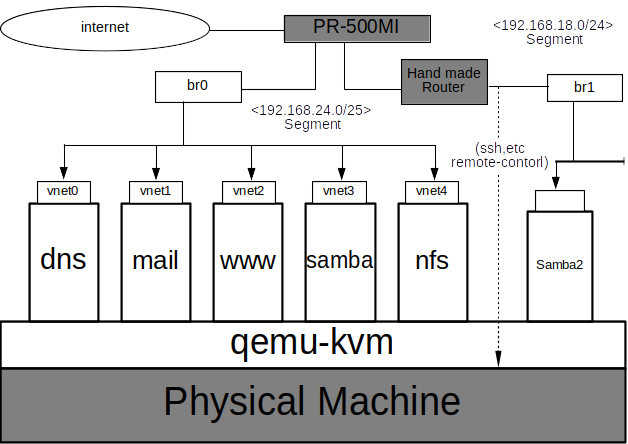
\includegraphics{image201803-kansai/external.png}
\caption{外部用ネットワークの図}
\end{figure*}
\clearpage

\subsubsection{外部用ネットワークの設定}
外部用のネットワークでの各VMのネットワークデバイスの設定は、第一にvirt-managerを使い仮想ネットワークを接続する仮想bridgeを作成します。次にVMのネットワークインターフェイスは、qemuでエミュレートされるTAPデバイスを作成して、単純に入出力を接続する「tap」を作ります。このtapは擬似的なethernetデバイスでLinuxカーネルの機能です。この仮想的なethernetデバイスを、同じくLinuxのカネールの機能である仮想bridgeで接続するこで、VMは実デバイスやほかのVMと接続することができます。

ただし、virt-managerで作成する仮想bridgeはdefaultでサブネットを設定できません。なので、interfacesファイルを直接、編集してサブネットを設定します。また、Hand made Router、VMのDNSの両方にbindパッケージをインストールし、外部用ネットワークを構築します。

次に、Hand made Routerはルータにするために、iptablesとiptables-persistenのパッケージを使います。また、/etc/sysctl.confのnet.ipv4.ip_forward=1のコメントを外しておきます。具体的には

\begin{itemize}
\item 仮想bridge、Hand made Routerでのサブネットの設定\\
VMを走らせる実機は qemu-kvm virt-managerをインストールして設定します。そして同機の/etc/network/interfacesを以下のように直接、編集します。
\begin{commandline}
# The loopback network interface
auto lo
iface lo inet loopback

# The primary network interface
allow-hotplug br0
iface br0 inet static
   address 192.168.24.108
   netmask 255.255.255.128
   gateway 192.168.24.1
   bridge_ports enp9s0
   bridge_stp on
   bridge_fd 0.0
# This is an autoconfigured IPv6 interface
iface enp9s0 inet6 auto

# The secondary network interface
auto enx0022cf56e5ca
allow-hotplug enx0022cf56e5ca
iface enx0022cf56e5ca inet static
address 192.168.18.80
netmask 255.255.255.0
gateway 192.168.18.80
# This is an autoconfigured IPv6 interface
iface enx0022cf56e5ca inet6 auto
\end{commandline}
次にHand made Routerはルータとして機能し、VMのモニターと保守も行い、インターネットからの入口にもします。設定としては /etc/network/interfacesと/etc/iptables/rules.v4を以下の様にします。\\
--------interfaces--------
\begin{commandline}
# The loopback network interface
auto lo
iface lo inet loopback

# The primary network interface
auto enp2s1
allow-hotplug enp2s1
iface enp2s1 inet static
address 192.168.24.88
netmask 255.255.255.128
gateway 192.168.24.1

# This is an autoconfigured IPv6 interface
iface enp2s1 inet6 auto

# The secondary network interface
allow-hotplug ens32
iface ens32 inet static
address 192.168.18.1
netmask 255.255.255.0
gateway 192.168.18.1

# This is an autoconfigured IPv6 interface
iface ens32 inet6 auto
\end{commandline}
\clearpage
--------rules.v4--------
\begin{commandline}
# Generated by iptables-save v1.6.0 on Sat Nov 18 17:30:00 2017
*filter
:INPUT ACCEPT [0:0]
:FORWARD ACCEPT [0:0]
:OUTPUT ACCEPT [0:0]

-A INPUT -i lo -j ACCEPT
...(Omltted)...
-A INPUT -i enp2s1 -m state --state RELATED,ESTABLISHED -j ACCEPT
-A INPUT -i enp2s1 -j DROP
...(Omltted)...
-A FORWARD -o ens32 -j REJECT --reject-with icmp-port-unreachable
-A FORWARD -i enp2s1 -m state --state RELATED,ESTABLISHED -j ACCEPT
-A FORWARD -o ens32 -m state --state NEW,ESTABLISHED -j ACCEPT

-A FORWARD -i enp2s1 -j DROP
-A FORWARD -o ens32 -j DROP

-A OUTPUT -o lo -j ACCEPT
...(Omltted)...
-A OUTPUT -o ens32 -m state --state NEW,ESTABLISHED -j ACCEPT
-A OUTPUT -o ens32 -j DROP
COMMIT
# Completed on Sat Mar 25 17:12:38 2017

# Generated by iptables-save v1.6.0 on Sat Apr 29 10:00:07 2017
*mangle
:PREROUTING ACCEPT [0:0]
:INPUT ACCEPT [0:0]
:FORWARD ACCEPT [0:0]
:OUTPUT ACCEPT [0:0]
:POSTROUTING ACCEPT [0:0]
-A POSTROUTING -o ens32 -p udp -m udp --dport 68 -j CHECKSUM --checksum-fill
COMMIT
# Completed on Sat Aug 26 16:07:34 2017

# Generated by iptables-save v1.4.21 on Sat Aug 26 16:07:34 2017
*nat
:PREROUTING ACCEPT [0:0]
:INPUT ACCEPT [0:0]
:OUTPUT ACCEPT [0:0]
:POSTROUTING ACCEPT [0:0]

-A POSTROUTING -s 192.168.18.0/24 ! -d 192.168.18.0/24 -j SNAT --to-source 192.168.24.88
COMMIT
# Completed on Sat Nov 18 17:30:00 2017
\end{commandline}

\clearpage

\item bindの各ステータスを使った外部用ネットワークの設定\\
 VMのDNS、Hand Made Routerにインストールするbindパッケージのnamed.confの設定方法は下図の通り。概要としては設定ファイルのnamed.confにincludeステーメントを使い、aclステートメント、optionsステートメントの設定ファイルを挿入します。同様にviewステートメントで、条件付けファイルによる動作を定義し、includeステートメントで条件ファイルを挿入します。
%図形の挿入
\begin{figure*}[!h]
\centering
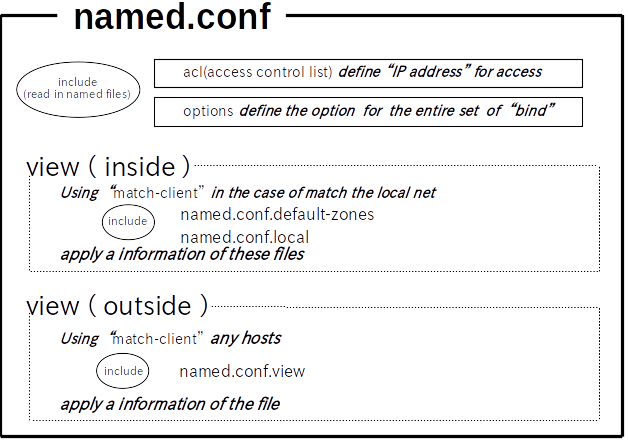
\includegraphics{image201803-kansai/named_conf.png}
\caption{named.confの図}
\end{figure*}

以下、各設定ファイルの詳細です。
\clearpage

\item named.conf(bindの設定ファイル)
\begin{commandline}
// This is the primary configuration file for the BIND DNS server named.
//
// Please read /usr/share/doc/bind9/README.Debian.gz for information on the
// structure of BIND configuration files in Debian, *BEFORE* you customize
// this configuration file.
//
// If you are just adding zones, please do that in /etc/bind/named.conf.local

include "/etc/bind/named.conf.acl";
include "/etc/bind/named.conf.options";

view "internal"{
	match-clients { localnet; };
	recursion yes;

include "/etc/bind/named.conf.local";
include "/etc/bind/named.conf.default-zones";

};

view "external" {
	match-clients { any; };
	recursion no;

include "/etc/bind/named.conf.view";

};
\end{commandline}
各ステートメントごとの設定ファイルは以下のようになります。\\

\item aclステートメント(アクセスするネットワークのIPアドレスの設定ファイル)
\begin{commandline}
acl localnet{
	192.168.24.0/25;
	192.168.24.128/26;
	192.168.24.192/26;
	192.168.18.0/24;
	127.0.0.1;
};
\end{commandline}

\item optionsステートメント(オプションでbind全体の動作を設定する)
\begin{commandline}
options {
	directory "/var/cache/bind";

	// If there is a firewall between you and nameservers you want
	// to talk to, you may need to fix the firewall to allow multiple
	// ports to talk.  See http://www.kb.cert.org/vuls/id/800113

	// If your ISP provided one or more IP addresses for stable
	// nameservers, you probably want to use them as forwarders.
	// Uncomment the following block, and insert the addresses replacing
	// the all-0's placeholder.

	forwarders {
	 	8.8.8.8; 8.8.4.4;
	};

	//========================================================================
	// If BIND logs error messages about the root key being expired,
	// you will need to update your keys.  See https://www.isc.org/bind-keys
	//========================================================================
	dnssec-validation auto;
	allow-query { any; };
        allow-transfer{
		localnet;
		8.8.8.8;
		8.8.4.4;
	};
	version "no version";
	auth-nxdomain no;    # conform to RFC1035
	listen-on-v6 { any; };
};
\end{commandline}
\clearpage

\item viweステートメント(内部)\\
  match-clientを使いローカルネットに以下の設定ファイルを適用する。\\
--- named.conf.default-zone ---
\begin{commandline}
// prime the server with knowledge of the root servers
zone "." {
	type hint;
	file "/etc/bind/db.root";
};

// be authoritative for the localhost forward and reverse zones, and for
// broadcast zones as per RFC 1912

zone "localhost" {
	type master;
	file "/etc/bind/db.local";
};

zone "127.in-addr.arpa" {
	type master;
	file "/etc/bind/db.127";
};

zone "0.in-addr.arpa" {
	type master;
	file "/etc/bind/db.0";
};

zone "255.in-addr.arpa" {
	type master;
	file "/etc/bind/db.255";
};
\end{commandline}
zoneステートメント(ホスト名とIPアドレスの対応関係のリストを定義する)で使われているこれらのファイルはdefaultでbindフォルダに含まれています。\\
--- named.conf.local ---
\begin{commandline}
//
// Do any local configuration here
//
zone "kinsen.gr.jp" {
	type master;
	file "/etc/bind/db.in-kinsen.gr.jp";
};
zone "24.168.192.in-addr.arpa" {
	type master;
	file "/etc/bind/db.192.168.24";
};
zone "18.168.192.in-addr.arpa" {
	type master;
	file "/etc/bind/db.192.168.18";
};
// Consider adding the 1918 zones here, if they are not used in your
// organization
//include "/etc/bind/zones.rfc1918";
\end{commandline}
以上のファイルは以下の通りです。
\clearpage

--- db.in-kinsen.gr.jp ---
\begin{commandline}
;
; BIND data file for kinsen.gr.jp
;
$TTL	86400
@	IN     SOA      bandai.kinsen.gr.jp. root.bandai.kinsen.gr.jp. (
		              1         ; Serial
			   1800         ; Refresh
			    900         ; Retry
			 604800         ; Expire
			   1200 )       ; Negative Cache TTL

		IN      NS      dns

; localhost
localhost       IN      A       127.0.0.1
localhost       IN      AAAA    ::1

; Mail exchange
                IN      MX      0 mail.kinsen.gr.jp.
;
; Host entry
;
mizu0           IN      A       192.168.18.1
;               IN      AAAA    2001
mizu1           IN      A       192.168.18.2
;               IN      AAAA    2001
kamaba          IN      A       192.168.18.80
;               IN      AAAA    2001
noren           IN      A       192.168.24.108
;               IN      AAAA    2001
dns             IN      A       192.168.24.81
;               IN      AAAA    2001:
mail            IN      A       192.168.24.82
;               IN      AAAA    2001:
www             IN      A       192.168.24.83
;               IN      AAAA    2001:
karan           IN      A       192.168.24.84
;               IN      AAAA    2001:
datuiba         IN      A       192.168.24.85
;               IN      AAAA    2001:
bandai          IN      A       192.168.24.88
;               IN      AAAA    2001:
yubune          IN      A       192.168.24.18
;               IN      AAAA    2001:
;
; Alias
;www            IN      CNAME    noren
;
; Domain
@               IN      A       192.168.24.88
                IN      MX 0    mail
\end{commandline}
--- db.192.168.24 ---
\begin{commandline}
;
; BIND data file for 192.168.24 network
;
$TTL	86400
@         IN    SOA     bandai.kinsen.gr.jp. root.bandai.kinsen.gr.jp. (
		              1         ; Serial
			   1800         ; Refresh
			    900         ; Retry
			 604800         ; Expire
			   1200 )       ; Negative Cache TTL

                IN      NS      dns
;
; Host entry
;
108             IN      PTR     noren.kinsen.gr.jp.
81              IN      PTR     dns.kinsen.gr.jp.
82              IN      PTR     mail.kinsen.gr.jp.
83              IN      PTR     www.kinsen.gr.jp.
84              IN      PTR     karan.kinsen.gr.jp.
85              IN      PTR     datuiba.kinsen.gr.jp.
88              IN      PTR     bandai.kinsen.gr.jp.
18              IN      PTR     yubune.kinsen.gr.jp.
\end{commandline}
\clearpage

\item viewステートメント(外部)\\
  match-clientを使いすべての外部hostにnamed.conf.viewファイルを適用する。\\
--- named.conf.view ---
\begin{commandline}
zone "." {
	type hint;
	file "/etc/bind/db.root";
};
zone "kinsen.gr.jp"{
	type master;
	file "/etc/bind/db.out-kinsen.gr.jp";
};
zone "158.141.203.in-addr.arpa"{
	type master;
	file "/etc/bind/db.203.141.158";
};
\end{commandline}
db.rootファイルはdefaultでbindフォルダにあります。out-kinsen.gr.jp、db.203.141.158については以下の通り。\\
--- out-kinsen.gr.jp ---
\begin{commandline}
;
; BIND data file for kinsen.gr.jp
;
$TTL	86400
@        IN      SOA    bandai.kinsen.gr.jp. root.bandai.kinsen.gr.jp. (
                              1         ; Serial
			   1800         ; Refresh
			    900         ; Retry
			 604800         ; Expire
			   1200 )       ; Negative Cache TTL
                                   
                IN   NS       dns

; localhost
localhost       IN      A       127.0.0.1
localhost       IN      AAAA    ::1

; Mail exchange
                IN      MX      0 mail.kinsen.gr.jp.
;
; Host entry
;
noren           IN      A       203.141.158.41
;               IN      AAAA    2001:
dns             IN      A       203.141.158.41
;               IN      AAAA    2001:
mail            IN      A       203.141.158.41
;               IN      AAAA    2001:
www             IN      A       203.141.158.41
;               IN      AAAA    2001:
karan           IN      A       203.141.158.41
;               IN      AAAA    2001:
datuiba         IN      A       203.141.158.41
;               IN      AAAA    2001:
bandai          IN      A       203.141.158.41
;               IN      AAAA    2001:
yubune          IN      A       203.141.158.41
;               IN      AAAA    2001:
;
; Domain
@               IN      A       203.141.158.41
                IN      MX 0    mail
\end{commandline}
\clearpage

--- db.203.141.58 ---
\begin{commandline}
;
; BIND data file for 203.141.158 network
;
$TTL    86400
@       IN      SOA     bandai.kinsen.gr.jp. root.bandai.kinsen.gr.jp. (
                              1         ; Serial
                           1800         ; Refresh
                            900         ; Retry
                         604800         ; Expire
                           1200 )       ; Negative Cache TTL

                  IN        NS      dns
;
; Host entry
;
41		IN	PTR	noren.kinsen.gr.jp.
41		IN	PTR	dns.kinsen.gr.jp.
41		IN	PTR	mail.kinsen.gr.jp.
41		IN	PTR	www.kinsen.gr.jp.
41		IN	PTR	karan.kinsen.gr.jp.
41		IN	PTR	datuiba.kinsen.gr.jp.
41		IN	PTR	bandai.kinsen.gr.jp.
41		IN	PTR	yubune.kinsen.gr.jp.
\end{commandline}
\end{itemize}

\subsection{内部用ネットワーク}
\subsubsection{内部用ネットワークの概要}
内部用ネットワークは実機PCに仮想ルータを作り、Wifi経由で実機上で走るVMをプライベートネットを3に分けたそれぞれのセグメント(192.168.24.0/25 192.168.24.128/26 1923168.24.192/26)につなぎます。\\
概要は下図の通り。

%図形の挿入
\begin{figure*}[!h]
\centering
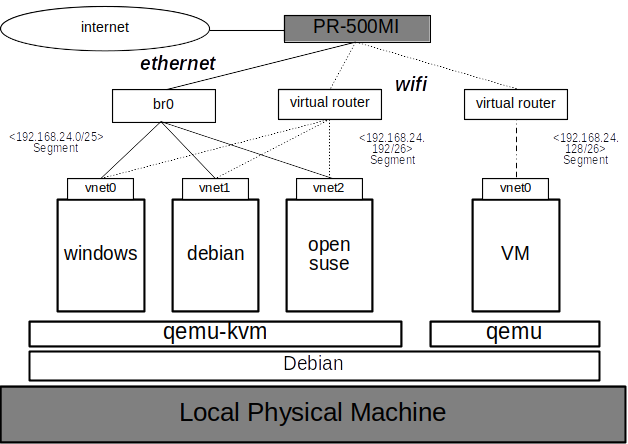
\includegraphics{image201803-kansai/internal.png}
\caption{内部用ネットワークの図}
\end{figure*}
\clearpage

\subsubsection{内部用ネットワークの設定}
内部用ネットワークの設定は、前提としてvirt-managerのConnection Detailsのvirtual networkで仮想ルータを作っておきます。また、実機PCをルータにする事を前提にしていますので、前述のHand made Routerのように、interfacesとrules.v4のファイルを以下のように設定します。

--- interfaces ---
\begin{commandline}
# This file describes the network interfaces available on your system
# and how to activate them. For more information, see interfaces(5).

source /etc/network/interfaces.d/*

# The loopback network interface
auto lo
iface lo inet loopback

# The primary network interface
allow-hotplug wlp1s0
iface  wlp1s0 inet dhcp

# This is an autoconfigured IPv6 interface
iface wlp1s0 inet6 auto

# The primary network interface
allow-hotplug enx0022cf56e5ca
iface br0 inet static
   address 192.168.24.8
   netmask 255.255.255.128
   gateway 192.168.24.1
   bridge_ports enx0022cf56e5ca
   bridge_stp on
   bridge_fd 0.0
# This is an autoconfigured IPv6 interface
iface enx0022cf56e5ca inet6 auto
iface br0 inet6 auto
\end{commandline}
\clearpage

--- rules.v4 ---
\begin{commandline}
# Generated by iptables-save v1.6.0 on Sat Apr 29 10:00:07 2017
*filter
:INPUT ACCEPT [0:0]
:FORWARD ACCEPT [0:0]
:OUTPUT ACCEPT [0:0]
-A INPUT -i lo -j ACCEPT
-A INPUT -i enx0022cf56e5ca -j ACCEPT
-A INPUT -i br0 -j ACCEPT

-A INPUT -i wlp1s0 -p udp -m udp --dport 123 -j ACCEPT
-A INPUT -i wlp1s0 -p udp -m udp --dport 53 -j ACCEPT
-A INPUT -i wlp1s0 -p tcp -m tcp --dport 53 -j ACCEPT
-A INPUT -i wlp1s0 -p udp -m udp --dport 67:68 -j ACCEPT
-A INPUT -i wlp1s0 -p tcp -m tcp --dport 80 -j ACCEPT
-A INPUT -i wlp1s0 -p tcp -m tcp --dport 443 -j ACCEPT
-A INPUT -i wlp1s0 -p udp -m udp --dport 111 -j ACCEPT
-A INPUT -i wlp1s0 -p tcp -m tcp --dport 111 -j ACCEPT
-A INPUT -i wlp1s0 -p udp -m udp --dport 2049 -j ACCEPT
-A INPUT -i wlp1s0 -p tcp -m tcp --dport 2049 -j ACCEPT
-A INPUT -i wlp1s0 -p udp -m udp --dport 445 -j ACCEPT
-A INPUT -i wlp1s0 -p tcp -m tcp --dport 445 -j ACCEPT
-A INPUT -i wlp1s0 -p tcp -m tcp --dport 5900:6000 -j ACCEPT
-A INPUT -i wlp1s0 -p udp -m udp --dport 32800:32805 -j ACCEPT
-A INPUT -i wlp1s0 -p tcp -m tcp --dport 32800:32805 -j ACCEPT
-A INPUT -i wlp1s0 -m state --state RELATED,ESTABLISHED -j ACCEPT
-A INPUT -i wlp1s0 -j DROP


-A FORWARD -i wlp1s0 -p udp -m udp --dport 123 -j ACCEPT
-A FORWARD -o virbr1 -p udp -m udp --sport 123 -m state --state ESTABLISHED -j ACCEPT
-A FORWARD -i wlp1s0 -p udp -m udp --dport 53 -j ACCEPT
-A FORWARD -o virbr1 -p udp -m udp --sport 53 -m state --state ESTABLISHED -j ACCEPT
-A FORWARD -i wlp1s0 -p tcp -m tcp --dport 53 -j ACCEPT
-A FORWARD -o virbr1 -p tcp -m tcp --sport 53 -m state --state ESTABLISHED -j ACCEPT
-A FORWARD -i wlp1s0 -p udp -m udp --dport 67 -j ACCEPT
-A FORWARD -o virbr1 -p udp -m udp --sport 67 -m state --state ESTABLISHED -j ACCEPT
-A FORWARD -i wlp1s0 -p udp -m udp --dport 68 -j ACCEPT
-A FORWARD -o virbr1 -p udp -m udp --sport 68 -m state --state ESTABLISHED -j ACCEPT
-A FORWARD -i wlp1s0 -p tcp -m tcp --dport 80 -j ACCEPT
-A FORWARD -o virbr1 -p tcp -m tcp --sport 80 -m state --state ESTABLISHED -j ACCEPT
-A FORWARD -i wlp1s0 -p tcp -m tcp --dport 443 -j ACCEPT
-A FORWARD -o virbr1 -p tcp -m tcp --sport 443 -m state --state ESTABLISHED -j ACCEPT
-A FORWARD -i wlp1s0 -p udp -m udp --dport 445 -j ACCEPT
-A FORWARD -o virbr1 -p udp -m udp --sport 445 -m state --state ESTABLISHED -j ACCEPT
-A FORWARD -i wlp1s0 -p tcp -m tcp --dport 445 -j ACCEPT
-A FORWARD -o virbr1 -p tcp -m tcp --sport 445 -m state --state ESTABLISHED -j ACCEPT
-A FORWARD -i wlp1s0 -p tcp -m tcp --dport 5900:6000 -j ACCEPT
-A FORWARD -o virbr1 -p tcp -m tcp --sport 5900:6000 -m state --state ESTABLISHED -j ACCEPT
-A FORWARD -o virbr1 -j REJECT --reject-with icmp-port-unreachable
-A FORWARD -i wlp1s0 -m state --state RELATED,ESTABLISHED -j ACCEPT
-A FORWARD -o virbr1 -m state --state NEW,ESTABLISHED -j ACCEPT
-A FORWARD -i wlp1s0 -j DROP
-A FORWARD -o virbr1 -j DROP

-A OUTPUT -o lo -j ACCEPT
-A OUTPUT -o br0 -j ACCEPT

-A OUTPUT -o virbr1 -p udp -m udp --sport 123 -j ACCEPT
-A OUTPUT -o virbr1 -p udp -m udp --sport 53 -j ACCEPT
-A OUTPUT -o virbr1 -p tcp -m tcp --sport 53 -j ACCEPT
-A OUTPUT -o virbr1 -p udp -m udp --sport 67:68 -j ACCEPT
-A OUTPUT -o virbr1 -p tcp -m tcp --sport 80 -j ACCEPT
-A OUTPUT -o virbr1 -p tcp -m tcp --sport 443 -j ACCEPT
-A OUTPUT -o virbr1 -p udp -m udp --sport 111 -j ACCEPT
-A OUTPUT -o virbr1 -p tcp -m tcp --sport 111 -j ACCEPT
-A OUTPUT -o virbr1 -p udp -m udp --sport 2049 -j ACCEPT
-A OUTPUT -o virbr1 -p tcp -m tcp --sport 2049 -j ACCEPT
-A OUTPUT -o virbr1 -p udp -m udp --sport 445 -j ACCEPT
-A OUTPUT -o virbr1 -p tcp -m tcp --sport 445 -j ACCEPT
-A OUTPUT -o virbr1 -p tcp -m tcp --sport 5900:6000 -j ACCEPT
-A OUTPUT -o virbr1 -p udp -m udp --sport 32800:32805 -j ACCEPT
-A OUTPUT -o virbr1 -p tcp -m tcp --sport 32800:32805 -j ACCEPT
-A OUTPUT -o virbr1 -m state --state NEW,ESTABLISHED -j ACCEPT
-A OUTPUT -o virbr1 -j DROP
COMMIT

*mangle
:PREROUTING ACCEPT [0:0]
:INPUT ACCEPT [0:0]
:FORWARD ACCEPT [0:0]
:OUTPUT ACCEPT [0:0]
:POSTROUTING ACCEPT [0:0]
-A POSTROUTING -o virbr1 -p udp -m udp --dport 68 -j CHECKSUM --checksum-fill
COMMIT

*nat
:PREROUTING ACCEPT [0:0]
:INPUT ACCEPT [0:0]
:OUTPUT ACCEPT [0:0]
:POSTROUTING ACCEPT [0:0]
-A POSTROUTING -s 192.168.1.128/26 ! -d 192.168.1.128/26 -j MASQUERADE
-A POSTROUTING -s 192.168.1.192/26 ! -d 192.168.1.192/26 -j MASQUERADE
COMMIT
# Completed on Sat Jul 22 20:16:41 2017
\end{commandline}

\subsection{まとめ}
以上が、「我が家の仮想ネットワーク」の内容です。ただ、実際のところ本来のシンクライアントの目的からはズレています。今後はv6のへの対応や、OSサーバなるもの用意して、更なる”利便性”を追求するつもりです。

%201803 tokyo
\dancersection{go / debian での機械学習環境構築について}{ysaito}
%-------------------------------------------------------------------------------

\subsection{はじめに}
機械学習という分野では, python, あるいは, R が人気を二分する.
しかし, 第三の選択肢として, Go による機械学習環境がある.
Go で機械学習を行うメリットは, 静的型安全や, goroutine, channel, などの並行処理のメリットがあるが, 最も注目すべき点は, インフラ, システムプログラミングに対する親和性であると考える.

今回は, 機械学習そのものの解説には踏み込まず, Go/Debian による機械学習環境の構築に触れたい.

環境は debian 9.4 (stretch) を利用する.

\subsection{書籍の紹介}
Machine Learning With Go (Packt publishing)

\url{https://www.packtpub.com/big-data-and-business-intelligence/machine-learning-go}

\subsection{kuberetes, docker の準備}
VMサポートは, 有効にせずローカルでの実行を前提として minikube を導入する.

docker リポジトリの導入
\begin{commandline}
sudo apt install curl apt-transport-https ca-certificates software-properties-common
curl -fsSL https://download.docker.com/linux/debian/gpg | sudo apt-key add -
\end{commandline}

fingerprint の確認
\begin{commandline}
apt-key fingerprint 0EBFCD88

pub   rsa4096 2017-02-22 [SCEA]
      9DC8 5822 9FC7 DD38 854A  E2D8 8D81 803C 0EBF CD88
uid           [ unknown] Docker Release (CE deb) <docker@docker.com>
sub   4096R/F273FCD8 2017-02-22 [S]
\end{commandline}

docker の導入
\begin{commandline}
sudo apt install docker-ce
docker version
Docker version 18.03.0-ce, build 0520e24

# 入力データを処理するアルゴリズムがのった docker image を導入する
docker pull dwhitena/goregtrain:single
\end{commandline}


minikube の導入
\begin{commandline}
curl -Lo minikube https://storage.googleapis.com/minikube/releases/latest/minikube-linux-amd64 && \
chmod +x minikube && sudo mv minikube /usr/local/bin/

minikube version
minikube version v0.28.2
\end{commandline}

kubernetes リポジトリの導入
\begin{commandline}
curl -s https://packages.cloud.google.com/apt/doc/apt-key.gpg | sudo apt-key add -

#fingerprint の確認
apt-key fingerprint BA07F4FB

pub   rsa2048 2018-04-01 [SCEA] [expires: 2021-03-31]
      54A6 47F9 048D 5688 D7DA  2ABE 6A03 0B21 BA07 F4FB
uid           [ unknown] Google Cloud Packages Automatic Signing Key <gc-team@google.com>

# レポジトリ登録
cat <<EOF >/etc/apt/sources.list.d/kubernetes.list
deb http://apt.kubernetes.io/ kubernetes-xenial main
EOF
sudo apt update && sudo apt install kubectl
\end{commandline}


minikube 用の設定と minikube の開始
\begin{commandline}
export MINIKUBE_WANTUPDATENOTIFICATION=false
export MINIKUBE_WANTREPORTERRORPROMPT=false
export MINIKUBE_HOME=$HOME
export CHANGE_MINIKUBE_NONE_USER=true
mkdir $HOME/.kube || true
touch $HOME/.kube/config

export KUBECONFIG=$HOME/.kube/config

# vm-driver デフォルトでは VirtualBox 上に
# VM を構築し kuberuentes を構築する
# "none" を指定することで実行したマシン上に直接
# kubernetes を構築する
sudo minikube start --vm-driver=none

\end{commandline}

pachyderm の導入
\begin{commandline}
curl -o /tmp/pachctl.deb -L \
https://github.com/pachyderm/pachyderm/releases/download/v1.7.0rc4/pachctl_1.7.0rc4_amd64.deb && \
sudo dpkg -i /tmp/pachctl.deb

pachctl deploy local
\end{commandline}

\subsection{pachyderm とは}
pachydermとは, データのバージョン管理や, 機械学習の処理をパイプラインでつなぐことができる go 製のソフトウェアである.
詳しくは, \url{https://pachyderm.io} にて情報がある.

\subsection{構成する概要}

diabetes.csv から, go による機械学習アルゴリズムにより、モデル(csvから得られた関数のパラメータ)を生成し, model.json
新規に得られた入力, 1.json から予測, 1.json を出力する

\begin{commandline}
     +-------------------------------------------------------------+
     |                                                             |
     |                                                             |
     |  +----------+    +----------+    +------------+             |
     |  |          |    |          |    |            |             |
     |  |  学   習 |   | モ デ ル |    |  モ  デ  ル|             |
     |  |          |    |          |    |            |             |
+-----> |          +--> |          |--> |            |             |
     |  diabetes.csv    | ./goregtrain  | model.json |             |
     |  |          |    |          |    |            |             |
     |  +----------+    +----------+    +-----+------+             |
     |                                        |                    |
     |                  +----------+    +-----v------+  +--------+ |
     |                  |          |    |            |  |        | |
     |                  | attributes    | 予  測     |  | 予  測 | |
 +--------------------> |          +--> |            +> |        | |
     |                  |          |    |            |  |        | |
     |                  | 1.json   |    | ./goregpredict| 1.json | |
     |                  +----------+    +------------+  +--------+ |
     |                                                             |
     +-------------------------------------------------------------+
\end{commandline}

\subsection{入力に使用するデータ}
\url{https://github.com/PacktPublishing/Machine-Learning-With-Go/tree/master/Chapter09/building_a_scalable_pipeline/example2}

\subsection{go によって pachyderm へ接続しリポジトリを作る}
\begin{commandline}
// localhost 上の Kubernetes クラスタの pachyderm へ接続する
// デフォルトの pachyderm のポート 30650
c, err := client.NewFromAddress("0.0.0.0:30650")
if err != nil {
log.Fatal(err)
}
defer c.Close()
// 学習用のリポジトリを作成 "training."
if err := c.CreateRepo("training"); err != nil {
log.Fatal(err)
}
// 予測の入力用のリポジトリを作成する "attributes."
if err := c.CreateRepo("attributes"); err != nil {
log.Fatal(err)
}
// 2つのリポジトリに sanity check をおこなう
repos, err := c.ListRepo(nil)
if err != nil {
log.Fatal(err)
}
// リポジトリの数を確認する
if len(repos) != 2 {
log.Fatal("Unexpected number of data repositories")
}
\end{commandline}

コンパイルと実行
\begin{commandline}
go build
./create
pachctl list-repo
NAME CREATED SIZE
attributes 3 seconds ago 0B
training 3 seconds ago 0B
\end{commandline}

\subsection{attribute リポジトリ, training リポジトリへデータをセットする}

\begin{commandline}
// Pachyderm へ接続する
c, err := client.NewFromAddress("0.0.0.0:30650")
if err != nil {
log.Fatal(err)
}
defer c.Close()
// "attributes" データリポジトリにデータを "master" ブランチにコミットする処理を始める
commit, err := c.StartCommit("attributes", "master")
if err != nil {
log.Fatal(err)
}
// attributes に入れる JSON を開く
f, err := os.Open("1.json")
if err != nil {
log.Fatal(err)
}
// attributes へファイルをプットする
if _, err := c.PutFile("attributes", commit.ID, "1.json", f); err != nil {
log.Fatal(err)
}
// コミットを完了させる.
if err := c.FinishCommit("attributes", commit.ID); err != nil {
log.Fatal(err)
}
// "training" データリポジトリの "master" ブランチへデータをコミットする処理を始める.
commit, err = c.StartCommit("training", "master")
if err != nil {
log.Fatal(err)
}
// 学習用のデータセットファイルを開く
f, err = os.Open("diabetes.csv")
if err != nil {
log.Fatal(err)
}
// training データセットを 学習用データリポジトリに展開する.
if _, err := c.PutFile("training", commit.ID, "diabetes.csv", f); err !=
nil {
log.Fatal(err)
}
// コミットを完了させる.
if err := c.FinishCommit("training", commit.ID); err != nil {
log.Fatal(err)
}
\end{commandline}

コンパイルして実行する
\begin{commandline}
# 上記のコードをコンパイルする
go build
# 実行
./a

# リポジトリを表示する
pachctl list-repo
NAME CREATED SIZE
training 13 minutes ago 73.74KiB
attributes 13 minutes ago 210B

# training リポジトリの master ブランチのファイルを表示する
pachctl list-file training master
NAME TYPE SIZE
diabetes.csv file 73.74KiB

# attributes リポジトリの master ブランチのファイルを表示する
pachctl list-file attributes master
NAME TYPE SIZE
1.json file 210B
\end{commandline}

\subsection{model ステージのJSON を準備する}

\begin{commandline}
{
  "pipeline": {
    "name": "model"
  },
  "transform": {
    "image": "dwhitena/goregtrain:single",
    "cmd": [
      "/goregtrain",
      "-inDir=/pfs/training",
      "-outDir=/pfs/out"
    ]
  },
  "parallelism_spec": {
    "constant": "1"
  },
  "input": {
    "atom": {
      "repo": "training",
      "glob": "/"
    }
  }
}
\end{commandline}

\subsection{model ステージのJSON を準備する}

1.Pachyderm データパイプラインが model という名前であることを教える
2.Pachyderm へ, モデル作成に使うアルゴリズムを教える, docker イメージになっている線形回帰モデルを使用する( dwhitena/goregtrain:single ),
3. そして, 学習用データファイルとのパイプラインを教える

\begin{commandline}
# パイプラインの作成
pachctl create-pipeline -f model.json

# pods の状態確認
kubectl get pods
NAME READY STATUS RESTARTS AGE
etcd-2142892294-38ptw 1/1 Running 0 2h
pachd-776177201-04l6w 1/1 Running 0 2h
pipeline-model-v1-p0lnf 2/2 Running 0 1m

# pachyderm 上の job 確認
pachctl list-job
ID OUTPUT COMMIT STARTED DURATION RESTART PROGRESS DL UL STATE
14f052ae-878d-44c9-a1f9-ab0cf6d45227 model/a2c7b7dfb44a40e79318c2de30c7a0c8
3 minutes ago Less than a second 0 1 + 0 / 1 73.74KiB 160B success

# データリポジトリを確認
pachctl list-repo
NAME CREATED SIZE
model 3 minutes ago 160B
training About an hour ago 73.74KiB
attributes About an hour ago 210B

# model master ブランチにあるファイルを確認
pachctl list-file model master
NAME TYPE SIZE k8s
model.json file 160B

# model.json の中身を確認する
pachctl get-file model master model.json
{
  "intercept": 152.13348416289818,
  "coefficients": [
    {
      "name": "bmi",
      "coefficient": 949.4352603839862
    }
  ]
}
\end{commandline}


\subsection{予測用のパイプラインを設定し結果を得る}

\begin{commandline}
{
  "pipeline": {
    "name": "prediction"
  },
  "transform": {
    "image": "dwhitena/goregpredict",
    "cmd": [
      "/goregpredict",
      "-inModelDir=/pfs/model",
      "-inVarDir=/pfs/attributes",
      "-outDir=/pfs/out"
    ]
  },
  "parallelism_spec": {
    "constant": "1"
  },
  "input": {
    "cross": [
    {
      "atom": {
        "repo": "attributes",
        "glob": "/*"
      }
    },
      {
        "atom": {
          "repo": "model",
          "glob": "/"
        }
      }
    ]
  }
}
\end{commandline}

\begin{commandline}
# prediction.json へのデータパイプラインを作成する
pachctl create-pipeline -f prediction.json

# pachyderm 上の job のリストを確認する
pachctl list-job
ID OUTPUT COMMIT STARTED DURATION RESTART PROGRESS DL UL STATE
03f36398-89db-4de4-ad3d-7346d56883c0
prediction/5ce47c9e788d4893ae00c7ee6b1e8431 About a minute ago Less than a
second 0 1 + 0 / 1 370B 266B success
14f052ae-878d-44c9-a1f9-ab0cf6d45227 model/a2c7b7dfb44a40e79318c2de30c7a0c8
19 minutes ago Less than a second 0 1 + 0 / 1 73.74KiB 160B success

# リポジトリの確認をする
pachctl list-repo
NAME CREATED SIZE
prediction About a minute ago 266B
model 19 minutes ago 160B
training About an hour ago 73.74KiB
attributes About an hour ago 210B

# prediction リポジトリの master ブランチの中身を確認する
pachctl list-file prediction master
NAME TYPE SIZE
1.json file 266B

# 1.json ファイルの中身を確認する
pachctl get-file prediction master 1.json
\end{commandline}

%201804 kansai
%\dancersection{最近のDebianパッケージ作成環境 - git-buildpackage, sbuild, autopkgtest を例に -(資料無し)}{佐々木 洋平}

%201806 tokyo
%-------------------------------------------------------------------------------
\dancersection{salsaと東京エリアdebian勉強会のWeb/原稿システムの仕組み}{杉本 典充}
%-------------------------------------------------------------------------------

\subsection{はじめに}

東京エリアdebian勉強会では、勉強会を運営するにあたりwebサイトと勉強会の発表資料である原稿データとスライドデータを扱っています。これらのデータは勉強会の議論を深めたり記録として重要な資産になっています。


東京エリアDebian勉強会の資料の保存先を \url{salsa.debian.org} へ移行したため、資料を処理する仕組みとsalsaへの移行作業について報告します。


\subsection{東京エリアDebian勉強会のシステム}

東京エリアDebian勉強会では、運営を行うにあたり以下のシステムを利用しています。

\begin{itemize}
  \item webサイト「\url{https://tokyodebian-team.pages.debian.net/}」\footnote{リポジトリは、\url{https://salsa.debian.org/tokyodebian-team/tokyodebian-team.pages.debian.net}}
  \item 発表者の原稿データ、スライドデータを処理するtexの原稿システム\footnote{リポジトリは、\url{https://salsa.debian.org/tokyodebian-team/monthly-report}}
  \item 参加者申し込みとして外部サービス「connpass」\footnote{\url{https://connpass.com/}}
  \item DebianJPのメーリングリスト(勉強会の告知、相談、質問の窓口)
\end{itemize}


salsaを利用しているのは、webサイトと原稿データのファイル管理を行う必要な処理となります。


\subsection{salsa.debian.org}

\subsubsection{salsaとは}

salsaとは、Debianプロジェクトが \url{salsa.debian.org} として運用している開発者向けのプロジェクト管理サーバです。gitlabをインストールしたサーバになっており、現代のgitを使ったワークフローやKubernetes(k8s)と連携してCI/CDを実行する機能を持っています。


\subsubsection{aliothからsalsaへの移行}

Debianプロジェクトでは2003年から \url{alioth.debian.org} というプロジェクト管理サーバを運用していました。aliothはFusionForge\footnote{\url{http://www.fusionforge.org}}というOSSのwebベースなプロジェクト管理ツールをサービスするホストであり、webサーバ・wiki・メーリングリスト・CVS/SVN/GITのリポジトリをサービスしていました\footnote{https://wiki.debian.org/Alioth/FAQ\#FusionForge}。


しかし、FusionForgeは2016年12月10日に fusionforge-6.0.5 をリリースしてから開発が滞る状況になります。aliothサーバはDebian 7 (wheezy)にFusionForgeをインストールして運用していましたが、アプリケーションの更新が止まったことからaliothを今後どうしていくか議論が始まりました。


2017年8月17日にAlioth Sprint 2017を行い\footnote{https://wiki.debian.org/Sprints/2017/Alioth}、gitlabをベースにしたaliothの後継サーバのプロトタイプを実装し\footnote{https://wiki.debian.org/Salsa}、サーバ名を"salsa"と呼称することになります。


salsaは2017年12月15日にベータ運用に入り\footnote{salsa.debian.org (git.debian.org replacement) going into beta \url{https://lists.debian.org/debian-devel-announce/2017/12/msg00003.html}}、2018年1月27日にベータ運用を終了し本稼働を開始しました\footnote{salsa.debian.org updates (leaving beta) \url{https://lists.debian.org/debian-devel-announce/2018/01/msg00004.html}}。


そして、2018年5月31日のDebian 7 (wheezy) LTSの終了とともにaliothサーバはサービスを終了し、その機能をsalsaへ引き継ぎました。


\subsubsection{salsaの利用の仕方}

\subsubsubsection{ドキュメント}

salsaのドキュメントは以下にあります。Docのページにアカウントのセットアップからチームの作成までの流れが書いてあります。そのほか、gitlabのドキュメントを参照ください。

\begin{itemize}
  \item \url{https://wiki.debian.org/Salsa/}
  \item \url{https://wiki.debian.org/Salsa/Doc}
  \item \url{https://docs.gitlab.com/}
\end{itemize}

\subsubsubsection{アカウントの登録}

salsaはDebian Developerのユーザ管理を行うLDAPサーバと連携しています。そのため、Debian Developerの方はdebian.orgのメールアドレスを利用してsalsaへログインできます。


Debian Developer以外の方は、\url{https://signup.salsa.debian.org/} のページでsalsaのゲストアカウントを作成できます。このとき、ユーザアカウント名は"-guest"という文字列を末尾に含める命名規則になっています。


\subsubsubsection{チームの作成}

gitlab ではまず「チーム」というユーザのグループをつくり、チームの配下にプロジェクト群をつくる形になっています。

\url{https://signup.salsa.debian.org/} のページでチームを作成できます。チームの作成はDebian Developer以外の方でも可能です。チーム名は、"-team"という文字列を末尾に含める命名規則になっています。

チームを作成すると、例えば \url{https://salsa.debian.org/tokyodebian-team} のようなURLでチームのページにアクセスできるようになります。

なお、チームを作成したユーザは初期設定でチームのOwner権限を持ちます。


\subsubsubsection{チームへのメンバの参加}

salsaに存在するユーザアカウントをチームに追加することでプロジェクトの参加者を増やすことができます。ユーザの追加は、チームのOwnerまたはMasterの権限を持っているユーザが操作できます。

なおユーザ権限は \url{https://docs.gitlab.com/ee/user/permissions.html} に一覧があり、Owner、Master\footnote{\url{https://docs.gitlab.com/ee/user/permissions.html}のマニュアルではMaintainerになっていますが、salsaではMasterになっています。}、Developer、Reporter、Guestの権限があります。

また、自分がとあるチームへ参加したい場合は、salsaへログインした状態でチームのトップページにある「アクセス権限をリクエストする」ボタンを押下してください。するとチームへの追加依頼がチームの管理者へ通知され、許可されればチームのメンバに追加されます。


\subsubsubsection{プロジェクトの作成(=gitリポジトリの作成)}

チームのページの右上にある「+」マークの部分をクリックすると表示するメニューからプロジェクトを作成できます。

プロジェクト1つにつきgitリポジトリ1つを持つことができます。そのため、複数のgitリポジトリで構成するプロジェクトの場合は、チームが複数のプロジェクトをもつようにすることで実現できます。


\subsubsubsection{CI/CD}

gitlabはCI(Continuous Integration)やCD(Continuous Delivery)の機能を備えています。


ユーザがgitリポジトリへpushしたタイミングやwebhook\footnote{https://docs.gitlab.com/ee/user/project/integrations/webhooks.html}という仕組みを利用してCI/CDの処理を実行できます。主にユニットテストの自動実行や運用サーバへコミットしたファイルの自動配備、チャットへの通知などの処理を行うことが考えられます。


gitlabのCI/CD処理は、"Runner"というKubernetes(K8s)のインスタンスへ処理をリクエストする仕組みになっています。Runnerには、3つの種類があります\footnote{https://docs.gitlab.com/ee/ci/runners/}。

\begin{itemize}
\item Shared Runners\footnote{Runnerのサーバは不足しているためスポンサーを募集中です。\url{https://wiki.debian.org/Salsa/Doc\#Quick_start}}
  \begin{itemize}
  \item gitlabサーバの全チーム、全プロジェクト共用の汎用Runner。
  \item Kubernetesのバージョンやインスタンスを問わず実行してよい場合はこれを指定する。
  \end{itemize}
\item Group Runners
  \begin{itemize}
  \item 1つのチーム内のプロジェクト群のみで占有して利用できる汎用Runner。
  \end{itemize}
\item Specific Runners
  \begin{itemize}
  \item 1つのチーム内のプロジェクト群のみで占有して利用できる環境依存向けRunner。
  \item Runnerの動作環境に応じて1つまたは複数のタグを設定する。
  \item gitリポジトリの".gitlab-ci.yml"のtagsキーにタグを指定すると、指定したすべてのタグをもつSpecific RunnerへCI/CD処理の実行をリクエストする。
  \end{itemize}
\end{itemize}

gitlabのCI/CDは機能や設定項目も多いため、GitLabのマニュアル\footnote{https://docs.gitlab.com/ee/ci/README.html}を参照してください。


\subsubsubsection{ユーザ個人ページの設定}

ユーザの個人設定ページにある「SSH Keys」ページからSSH鍵を登録することができます。

SSH鍵を登録しておくと、gitのpullやpush時の認証でアカウントの入力をせずに済むため作業が効率化するでしょう。

salsaのgitリポジトリへpull、pushするユーザのホストには、以下のsshの接続設定をしておくとよいです。

\begin{commandline}
$ cat ~/.ssh/config
Host salsa.debian.org
  User youraccount-guest
  IdentityFile ~/.ssh/id_rsa.yoursalsakey
\end{commandline}


\subsection{東京エリアDebian勉強会のsalsaのシステム}

\subsubsection{aliothからsalsaへの移行の設計と作業内容}

東京エリアDebian勉強会(及び関西Debian勉強会)では、\url{alioth.debian.org} にあるgitリポジトリ及び静的ファイルのweb公開機能を使っていました。

2018年5月にaliothサーバが停止するため、salsaへgitリポジトリとwebサイトを移行するよう計画しました。システム移行の設計と実施する作業は以下URLにまとめています。

\begin{itemize}
  \item \url{https://wiki.debian.org/tokyodebian_salsa_migrate}
\end{itemize}


\subsubsection{ファイルのライセンス}

東京エリアDebian勉強会のgitリポジトリに収録しているファイルは、aliothに配置している時代からライセンスにGPLv2(またはGPLv3)を適用するルールとしています。勉強会に参加いただく方にはライセンスをご理解の上、コミットやパッチの提供をお願いいたします。


\subsubsection{チームとメンバ}

東京エリアDebian勉強会では、「tokyodebian-team」というチーム名にしています\footnote{https://salsa.debian.org/tokyodebian-team}。歴史的にaliothのプロジェクト名が"tokyodebian"になっていたため、そのまま引き継いでいます。\footnote{原稿システム部分については関西Debian勉強会の方々も共用しており、tokyoに限らずみなさん利用できます。}


tokyodebian-teamのメンバの権限をどう割り当てるかのポリシーは定めておらず、Owner権限を持つ方々に裁量を委ねる運用にしています。


gitリポジトリへのコミット権は不要で、原稿データやスライドデータをpatchで提供していただける方は、東京エリアDebian勉強会のwebサイトに「発表資料更新/提出方法」\footnote{\url{https://tokyodebian-team.pages.debian.net/prework-update.html}}というページがありますのでご参照いただき、patchを送信してください。


\subsubsection{静的ファイル公開機能:Pages}

salsaの静的ファイルをweb公開する「Pages」\footnote{\url{https://wiki.debian.org/Salsa/Doc\#Web_page_hosting}}という機能があります。


Pagesの機能では"https://\{namespace\}.pages.debian.net/\{project\}"というURLで静的ファイルのwebを公開できる仕様になっており、namespaceの部分にはチーム名が入ります。特例として、URLのホスト名と同名のプロジェクトを作った場合はproject部分のディレクトリを省略したURLを利用できます。これによりプロジェクト名を「tokyodebian-team.pages.debian.net」にすることで、Pagesで公開するURLを「\url{https://tokyodebian-team.pages.debian.net/}」にできます。


\subsubsection{webサイトの仕組み}

東京エリアDebian勉強会のwebサイトのソースコードは、\url{https://salsa.debian.org/tokyodebian-team/tokyodebian-team.pages.debian.net} のページにあります\footnote{関西Debian勉強会はDebian Wikiを使っています。\url{https://wiki.debian.org/KansaiDebianMeeting}}。


コンテンツはEmacs Muse\footnote{\url{https://www.gnu.org/software/emacs-muse/index.html}}を利用しており、htmlのテンプレートとデータから静的htmlを生成する仕組みになっています\footnote{github pagesで利用できるjekyllのようなツールです。}。


salsaでは、ソースコードであるmuseファイルをgit pushするとCI/CD処理を実行してmuseファイルからhtmlファイルを生成し、\url{https://tokyodebian-team.pages.debian.net/} へ自動配備するように処理しています。


CI/CD処理の設定ファイルは、gitリポジトリの".gitlab-ci.yml"\footnote{\url{https://salsa.debian.org/tokyodebian-team/tokyodebian-team.pages.debian.net/blob/master/.gitlab-ci.yml}}となります。


webサイトのコンテンツの構成は、東京エリアDebian勉強会のwebサイトに「このページを編集する方法について」\footnote{\url{https://tokyodebian-team.pages.debian.net/editing.html}}という裏方向けの説明ページがありますのでご参照ください。


\begin{figure}[H]
\begin{center}
  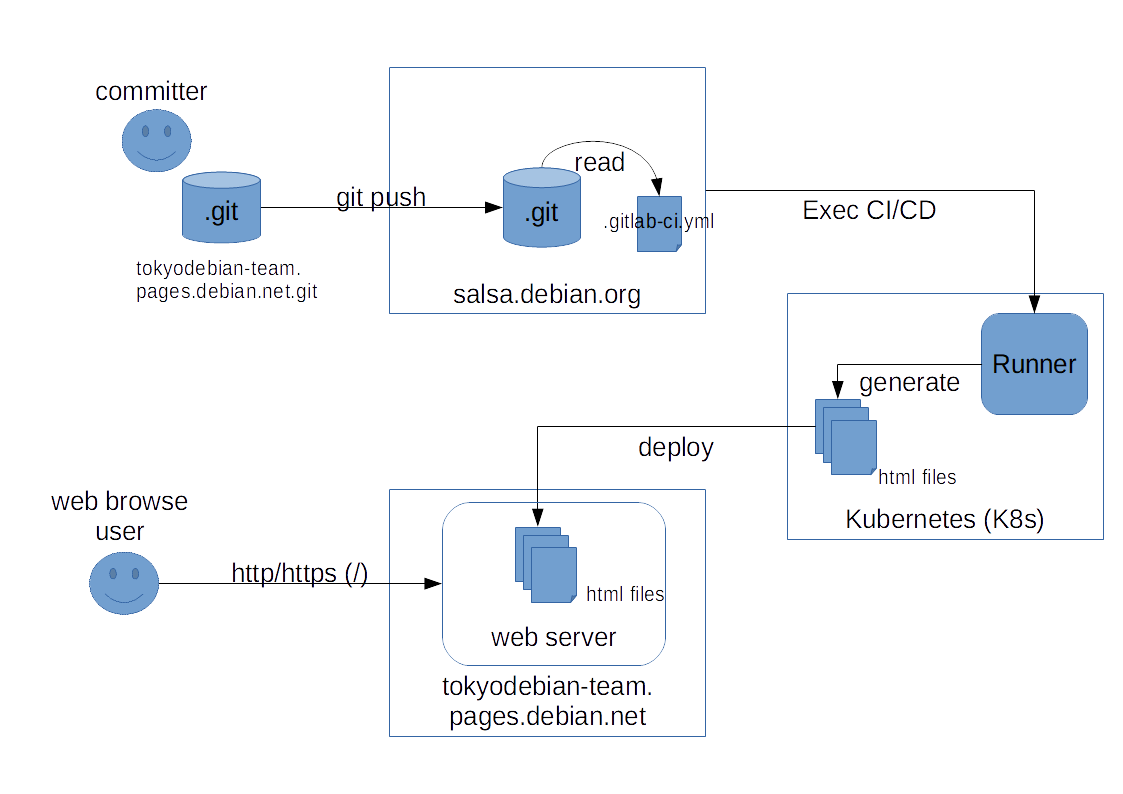
\includegraphics[width=12cm]{image201806/gitflow_web.png}
  \caption{webサイトへHTMLファイルを配備するCI/CD処理の流れ}
  \label{fig:deploy-html-CICD}
\end{center}
\end{figure}


\subsubsection{原稿システムの仕組み}

東京エリアDebian勉強会の原稿資料およびスライド資料のソースコードは、\url{https://salsa.debian.org/tokyodebian-team/monthly-report} のページにあります\footnote{関西Debian勉強会の資料もここにあります。}。


コンテンツはTeX(テフ)という組版システム\footnote{印刷を想定したレイアウトや文字、図などを配置して原稿を作成するシステムのことをいいます。}を利用しており、ソースコードであるtexファイルから中間ファイルのdviファイルを経て、最終的にpdfファイルを生成する仕組みになっています。配布している資料は、texのテンプレートを勉強会の有志が作成し、豊富な原稿の量は参加者の長年の積み重ねで支えられています。


salsaでは、texファイルを保存するgitリポジトリ"monthly-report.git"と、web公開するビルドしたpdfファイルを保存する"pdf20yy.git"というリポジトリに分けています\footnote{"pdf20xx.git"は、"pdf2005.git"から"pdf2018.git"まで存在しており、毎年増える予定です。}。これは、"monthly-report.git"でtexファイルをCI/CDの度にすべてビルドし直すには処理量が多すぎること、CI/CD処理が成功したとしてもpdfファイル数が多すぎてサーバ間のHTTP通信の送信可能サイズの上限を超えてエラーになることから\footnote{ERROR: Uploading artifacts to coordinator... too large archive id=11633 responseStatus=413 Request Entity Too Large status=413 Request Entity Too Large token=5ydbgD39}、一度のCI/CDで処理するpdfファイルの量を制限するためにリポジトリを年ごとに分割した経緯があります。


上記の転送ファイルサイズの制約を回避するため、salsaにおける原稿ファイルの生成からpdfファイルをweb公開するまでの処理は以下に流れになっています。


\begin{itemize}
  \item texファイルを保存している"monthly-report.git"をgit cloneしてtexファイルを作成する
  \item makeを実行し、pdfファイルが生成できることを確認する
  \item 原稿を完成させる
  \item texファイルをgit commitし、git pushする。push時にsalsaではCI/CD処理は実行しない
  \item make publishコマンドを実行し、pdfファイルを"pdf20yy.git"へgit commitし、git pushする
  \item "pdf20yy.git"でCI/CD処理を実行し、pdfファイルを"tokyodebian-team.pages.debian.net"に配備する
  \item webから"https://tokyodebian-team.pages.debian.net/pdf20yy/xxx.pdf"でファイルを取得できる
\end{itemize}


\begin{figure}[H]
\begin{center}
  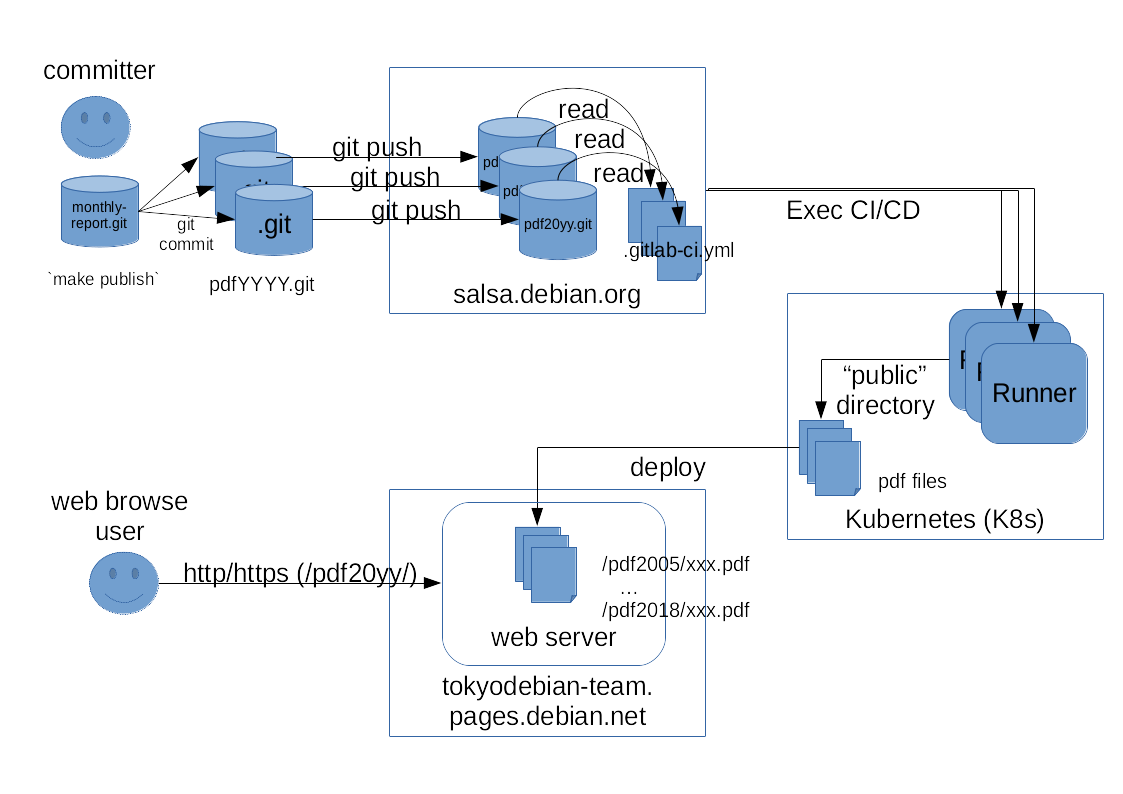
\includegraphics[width=12cm]{image201806/gitflow_pdf.png}
  \caption{webサイトへ原稿及びスライドPDFファイルを配備するCI/CD処理の流れ}
  \label{fig:deploy-pdf-CICD}
\end{center}
\end{figure}


\subsection{今後の課題}

原稿システムのCI/CD処理が失敗することもあり、Runnerや.gitlab-ci.ymlの設定を見直す必要があると考えています。

webサイトも原稿システムも作ってから年月が経過しているため、webサイトのリニューアルや原稿ファイルのUTF-8対応といった現代化をしていく重めの改修作業もあります。

また勉強会で発表していただいている方々も忙しいためか原稿を書いていただける方が減っており、半期のまとめ資料を冊子にしたときにページ数が少なくなってきている実情もあります。


\subsection{まとめ}

salsaで提供しているgitlabの機能と設定を紹介し、その機能を使って東京エリアDebian勉強会のシステムを移行した説明をしました。salsaを有効活用してDebianプロジェクトへ貢献することに繋がるとよいと思っています。

また、勉強会の参加者に原稿システムの理解を深めていただき、自分の学びになるだけでなく、他の参加者やインターネットで検索してきた方の学びにつながる勉強会にしていければよいと思っています。

%-------------------------------------------------------------------------------
% end of header
%-------------------------------------------------------------------------------

\clearpage
\newpage

%-------------------------------------------------------------------------------
%\dancersection{Debian Trivia Quiz}{野島 貴英}
%-------------------------------------------------------------------------------

%ところで、みなさん Debian 関連の話題においついていますか?Debian関連の話
%題はメーリングリストをよんでいると追跡できます。ただよんでいるだけではは
%りあいがないので、理解度のテストをします。特に一人だけでは意味がわからな
%いところもあるかも知れません。みんなで一緒に読んでみましょう。

%今回の出題範囲は\url{debian-devel-announce@lists.debian.org} や \url{debian-devel@lists.debian.org}に投稿された
%内容とDebian Project Newsからです。

%\begin{multicols}{2}
%\end{multicols}

% 索引
%\printindex
\clearpage
\begin{center}
本資料のライセンスについて
\end{center}

本資料はフリー・ソフトウェアです。あなたは、Free Software
Foundation が公表したGNU GENERAL PUBLIC LICENSEの "バージョン2"もしくはそれ以降
が定める条項に従って本プログラムを再頒布または変更することができ
ます。

本プログラムは有用とは思いますが、頒布にあたっては、市場性及び特
定目的適合性についての暗黙の保証を含めて、いかなる保証も行ないま
せん。詳細についてはGNU GENERAL PUBLIC LICENSE をお読みください。

\begin{multicols}{2}
 \begin{fontsize}{6}{6}
 \begin{verbatim}
            GNU GENERAL PUBLIC LICENSE
               Version 2, June 1991

 Copyright (C) 1989, 1991 Free Software Foundation, Inc.
    51 Franklin St, Fifth Floor, Boston, MA  02110-1301  USA
 Everyone is permitted to copy and distribute verbatim copies
 of this license document, but changing it is not allowed.

                Preamble

  The licenses for most software are designed to take away your
freedom to share and change it.  By contrast, the GNU General Public
License is intended to guarantee your freedom to share and change free
software--to make sure the software is free for all its users.  This
General Public License applies to most of the Free Software
Foundation's software and to any other program whose authors commit to
using it.  (Some other Free Software Foundation software is covered by
the GNU Library General Public License instead.)  You can apply it to
your programs, too.

  When we speak of free software, we are referring to freedom, not
price.  Our General Public Licenses are designed to make sure that you
have the freedom to distribute copies of free software (and charge for
this service if you wish), that you receive source code or can get it
if you want it, that you can change the software or use pieces of it
in new free programs; and that you know you can do these things.

  To protect your rights, we need to make restrictions that forbid
anyone to deny you these rights or to ask you to surrender the rights.
These restrictions translate to certain responsibilities for you if you
distribute copies of the software, or if you modify it.

  For example, if you distribute copies of such a program, whether
gratis or for a fee, you must give the recipients all the rights that
you have.  You must make sure that they, too, receive or can get the
source code.  And you must show them these terms so they know their
rights.

  We protect your rights with two steps: (1) copyright the software, and
(2) offer you this license which gives you legal permission to copy,
distribute and/or modify the software.

  Also, for each author's protection and ours, we want to make certain
that everyone understands that there is no warranty for this free
software.  If the software is modified by someone else and passed on, we
want its recipients to know that what they have is not the original, so
that any problems introduced by others will not reflect on the original
authors' reputations.

  Finally, any free program is threatened constantly by software
patents.  We wish to avoid the danger that redistributors of a free
program will individually obtain patent licenses, in effect making the
program proprietary.  To prevent this, we have made it clear that any
patent must be licensed for everyone's free use or not licensed at all.

  The precise terms and conditions for copying, distribution and
modification follow.

            GNU GENERAL PUBLIC LICENSE
   TERMS AND CONDITIONS FOR COPYING, DISTRIBUTION AND MODIFICATION

  0. This License applies to any program or other work which contains
a notice placed by the copyright holder saying it may be distributed
under the terms of this General Public License.  The "Program", below,
refers to any such program or work, and a "work based on the Program"
means either the Program or any derivative work under copyright law:
that is to say, a work containing the Program or a portion of it,
either verbatim or with modifications and/or translated into another
language.  (Hereinafter, translation is included without limitation in
the term "modification".)  Each licensee is addressed as "you".

Activities other than copying, distribution and modification are not
covered by this License; they are outside its scope.  The act of
running the Program is not restricted, and the output from the Program
is covered only if its contents constitute a work based on the
Program (independent of having been made by running the Program).
Whether that is true depends on what the Program does.

  1. You may copy and distribute verbatim copies of the Program's
source code as you receive it, in any medium, provided that you
conspicuously and appropriately publish on each copy an appropriate
copyright notice and disclaimer of warranty; keep intact all the
notices that refer to this License and to the absence of any warranty;
and give any other recipients of the Program a copy of this License
along with the Program.

You may charge a fee for the physical act of transferring a copy, and
you may at your option offer warranty protection in exchange for a fee.

  2. You may modify your copy or copies of the Program or any portion
of it, thus forming a work based on the Program, and copy and
distribute such modifications or work under the terms of Section 1
above, provided that you also meet all of these conditions:

    a) You must cause the modified files to carry prominent notices
    stating that you changed the files and the date of any change.

    b) You must cause any work that you distribute or publish, that in
    whole or in part contains or is derived from the Program or any
    part thereof, to be licensed as a whole at no charge to all third
    parties under the terms of this License.

    c) If the modified program normally reads commands interactively
    when run, you must cause it, when started running for such
    interactive use in the most ordinary way, to print or display an
    announcement including an appropriate copyright notice and a
    notice that there is no warranty (or else, saying that you provide
    a warranty) and that users may redistribute the program under
    these conditions, and telling the user how to view a copy of this
    License.  (Exception: if the Program itself is interactive but
    does not normally print such an announcement, your work based on
    the Program is not required to print an announcement.)

These requirements apply to the modified work as a whole.  If
identifiable sections of that work are not derived from the Program,
and can be reasonably considered independent and separate works in
themselves, then this License, and its terms, do not apply to those
sections when you distribute them as separate works.  But when you
distribute the same sections as part of a whole which is a work based
on the Program, the distribution of the whole must be on the terms of
this License, whose permissions for other licensees extend to the
entire whole, and thus to each and every part regardless of who wrote it.

Thus, it is not the intent of this section to claim rights or contest
your rights to work written entirely by you; rather, the intent is to
exercise the right to control the distribution of derivative or
collective works based on the Program.

In addition, mere aggregation of another work not based on the Program
with the Program (or with a work based on the Program) on a volume of
a storage or distribution medium does not bring the other work under
the scope of this License.

  3. You may copy and distribute the Program (or a work based on it,
under Section 2) in object code or executable form under the terms of
Sections 1 and 2 above provided that you also do one of the following:

    a) Accompany it with the complete corresponding machine-readable
    source code, which must be distributed under the terms of Sections
    1 and 2 above on a medium customarily used for software interchange; or,

    b) Accompany it with a written offer, valid for at least three
    years, to give any third party, for a charge no more than your
    cost of physically performing source distribution, a complete
    machine-readable copy of the corresponding source code, to be
    distributed under the terms of Sections 1 and 2 above on a medium
    customarily used for software interchange; or,

    c) Accompany it with the information you received as to the offer
    to distribute corresponding source code.  (This alternative is
    allowed only for noncommercial distribution and only if you
    received the program in object code or executable form with such
    an offer, in accord with Subsection b above.)

The source code for a work means the preferred form of the work for
making modifications to it.  For an executable work, complete source
code means all the source code for all modules it contains, plus any
associated interface definition files, plus the scripts used to
control compilation and installation of the executable.  However, as a
special exception, the source code distributed need not include
anything that is normally distributed (in either source or binary
form) with the major components (compiler, kernel, and so on) of the
operating system on which the executable runs, unless that component
itself accompanies the executable.

If distribution of executable or object code is made by offering
access to copy from a designated place, then offering equivalent
access to copy the source code from the same place counts as
distribution of the source code, even though third parties are not
compelled to copy the source along with the object code.

  4. You may not copy, modify, sublicense, or distribute the Program
except as expressly provided under this License.  Any attempt
otherwise to copy, modify, sublicense or distribute the Program is
void, and will automatically terminate your rights under this License.
However, parties who have received copies, or rights, from you under
this License will not have their licenses terminated so long as such
parties remain in full compliance.

  5. You are not required to accept this License, since you have not
signed it.  However, nothing else grants you permission to modify or
distribute the Program or its derivative works.  These actions are
prohibited by law if you do not accept this License.  Therefore, by
modifying or distributing the Program (or any work based on the
Program), you indicate your acceptance of this License to do so, and
all its terms and conditions for copying, distributing or modifying
the Program or works based on it.

  6. Each time you redistribute the Program (or any work based on the
Program), the recipient automatically receives a license from the
original licensor to copy, distribute or modify the Program subject to
these terms and conditions.  You may not impose any further
restrictions on the recipients' exercise of the rights granted herein.
You are not responsible for enforcing compliance by third parties to
this License.

  7. If, as a consequence of a court judgment or allegation of patent
infringement or for any other reason (not limited to patent issues),
conditions are imposed on you (whether by court order, agreement or
otherwise) that contradict the conditions of this License, they do not
excuse you from the conditions of this License.  If you cannot
distribute so as to satisfy simultaneously your obligations under this
License and any other pertinent obligations, then as a consequence you
may not distribute the Program at all.  For example, if a patent
license would not permit royalty-free redistribution of the Program by
all those who receive copies directly or indirectly through you, then
the only way you could satisfy both it and this License would be to
refrain entirely from distribution of the Program.

If any portion of this section is held invalid or unenforceable under
any particular circumstance, the balance of the section is intended to
apply and the section as a whole is intended to apply in other
circumstances.

It is not the purpose of this section to induce you to infringe any
patents or other property right claims or to contest validity of any
such claims; this section has the sole purpose of protecting the
integrity of the free software distribution system, which is
implemented by public license practices.  Many people have made
generous contributions to the wide range of software distributed
through that system in reliance on consistent application of that
system; it is up to the author/donor to decide if he or she is willing
to distribute software through any other system and a licensee cannot
impose that choice.

This section is intended to make thoroughly clear what is believed to
be a consequence of the rest of this License.

  8. If the distribution and/or use of the Program is restricted in
certain countries either by patents or by copyrighted interfaces, the
original copyright holder who places the Program under this License
may add an explicit geographical distribution limitation excluding
those countries, so that distribution is permitted only in or among
countries not thus excluded.  In such case, this License incorporates
the limitation as if written in the body of this License.

  9. The Free Software Foundation may publish revised and/or new versions
of the General Public License from time to time.  Such new versions will
be similar in spirit to the present version, but may differ in detail to
address new problems or concerns.

Each version is given a distinguishing version number.  If the Program
specifies a version number of this License which applies to it and "any
later version", you have the option of following the terms and conditions
either of that version or of any later version published by the Free
Software Foundation.  If the Program does not specify a version number of
this License, you may choose any version ever published by the Free Software
Foundation.

  10. If you wish to incorporate parts of the Program into other free
programs whose distribution conditions are different, write to the author
to ask for permission.  For software which is copyrighted by the Free
Software Foundation, write to the Free Software Foundation; we sometimes
make exceptions for this.  Our decision will be guided by the two goals
of preserving the free status of all derivatives of our free software and
of promoting the sharing and reuse of software generally.

                NO WARRANTY

  11. BECAUSE THE PROGRAM IS LICENSED FREE OF CHARGE, THERE IS NO WARRANTY
FOR THE PROGRAM, TO THE EXTENT PERMITTED BY APPLICABLE LAW.  EXCEPT WHEN
OTHERWISE STATED IN WRITING THE COPYRIGHT HOLDERS AND/OR OTHER PARTIES
PROVIDE THE PROGRAM "AS IS" WITHOUT WARRANTY OF ANY KIND, EITHER EXPRESSED
OR IMPLIED, INCLUDING, BUT NOT LIMITED TO, THE IMPLIED WARRANTIES OF
MERCHANTABILITY AND FITNESS FOR A PARTICULAR PURPOSE.  THE ENTIRE RISK AS
TO THE QUALITY AND PERFORMANCE OF THE PROGRAM IS WITH YOU.  SHOULD THE
PROGRAM PROVE DEFECTIVE, YOU ASSUME THE COST OF ALL NECESSARY SERVICING,
REPAIR OR CORRECTION.

  12. IN NO EVENT UNLESS REQUIRED BY APPLICABLE LAW OR AGREED TO IN WRITING
WILL ANY COPYRIGHT HOLDER, OR ANY OTHER PARTY WHO MAY MODIFY AND/OR
REDISTRIBUTE THE PROGRAM AS PERMITTED ABOVE, BE LIABLE TO YOU FOR DAMAGES,
INCLUDING ANY GENERAL, SPECIAL, INCIDENTAL OR CONSEQUENTIAL DAMAGES ARISING
OUT OF THE USE OR INABILITY TO USE THE PROGRAM (INCLUDING BUT NOT LIMITED
TO LOSS OF DATA OR DATA BEING RENDERED INACCURATE OR LOSSES SUSTAINED BY
YOU OR THIRD PARTIES OR A FAILURE OF THE PROGRAM TO OPERATE WITH ANY OTHER
PROGRAMS), EVEN IF SUCH HOLDER OR OTHER PARTY HAS BEEN ADVISED OF THE
POSSIBILITY OF SUCH DAMAGES.

             END OF TERMS AND CONDITIONS

        How to Apply These Terms to Your New Programs

  If you develop a new program, and you want it to be of the greatest
possible use to the public, the best way to achieve this is to make it
free software which everyone can redistribute and change under these terms.

  To do so, attach the following notices to the program.  It is safest
to attach them to the start of each source file to most effectively
convey the exclusion of warranty; and each file should have at least
the "copyright" line and a pointer to where the full notice is found.

    <one line to give the program's name and a brief idea of what it does.>
    Copyright (C) <year>  <name of author>

    This program is free software; you can redistribute it and/or modify
    it under the terms of the GNU General Public License as published by
    the Free Software Foundation; either version 2 of the License, or
    (at your option) any later version.

    This program is distributed in the hope that it will be useful,
    but WITHOUT ANY WARRANTY; without even the implied warranty of
    MERCHANTABILITY or FITNESS FOR A PARTICULAR PURPOSE.  See the
    GNU General Public License for more details.

    You should have received a copy of the GNU General Public License
    along with this program; if not, write to the Free Software
    Foundation, Inc., 51 Franklin St, Fifth Floor, Boston, MA  02110-1301 USA


Also add information on how to contact you by electronic and paper mail.

If the program is interactive, make it output a short notice like this
when it starts in an interactive mode:

    Gnomovision version 69, Copyright (C) year  name of author
    Gnomovision comes with ABSOLUTELY NO WARRANTY; for details type `show w'.
    This is free software, and you are welcome to redistribute it
    under certain conditions; type `show c' for details.

The hypothetical commands `show w' and `show c' should show the appropriate
parts of the General Public License.  Of course, the commands you use may
be called something other than `show w' and `show c'; they could even be
mouse-clicks or menu items--whatever suits your program.

You should also get your employer (if you work as a programmer) or your
school, if any, to sign a "copyright disclaimer" for the program, if
necessary.  Here is a sample; alter the names:

  Yoyodyne, Inc., hereby disclaims all copyright interest in the program
  `Gnomovision' (which makes passes at compilers) written by James Hacker.

  <signature of Ty Coon>, 1 April 1989
  Ty Coon, President of Vice

This General Public License does not permit incorporating your program into
proprietary programs.  If your program is a subroutine library, you may
consider it more useful to permit linking proprietary applications with the
library.  If this is what you want to do, use the GNU Library General
Public License instead of this License.
 \end{verbatim}
 \end{fontsize}
\end{multicols}

\begin{center}
ソースコードについて
\end{center}

このプログラムは tex で記述されたものです。ソースコードは
\begin{center}
  \url{git://anonscm.debian.org/tokyodebian/monthly-report.git}
\end{center}
から取得できます。

\begin{center}
Debian オープンユーズロゴ ライセンス
\end{center}

\begin{multicols}{2}
 \begin{fontsize}{6}{6}
 \begin{verbatim}

Copyright (c) 1999 Software in the Public Interest
Permission is hereby granted, free of charge, to any person
obtaining a copy of this software and associated documentation
files (the "Software"), to deal in the Software without restriction,
including without limitation the rights to use, copy, modify, merge,
publish, distribute, sublicense, and/or sell copies of the Software,
and to permit persons to whom the Software is furnished to do so,
subject to the following conditions:

The above copyright notice and this permission notice shall be
included in all copies or substantial portions of the Software.

THE SOFTWARE IS PROVIDED "AS IS", WITHOUT WARRANTY OF ANY
KIND, EXPRESS OR IMPLIED, INCLUDING BUT NOT LIMITED TO THE
WARRANTIES OF MERCHANTABILITY, FITNESS FOR A PARTICULAR PURPOSE AND
NONINFRINGEMENT. IN NO EVENT SHALL THE AUTHORS OR COPYRIGHT HOLDERS
BE LIABLE FOR ANY CLAIM, DAMAGES OR OTHER LIABILITY, WHETHER IN
AN ACTION OF CONTRACT, TORT OR OTHERWISE, ARISING FROM, OUT OF OR
IN CONNECTION WITH THE SOFTWARE OR THE USE OR OTHER DEALINGS IN
THE SOFTWARE.
 \end{verbatim}
 \end{fontsize}
\end{multicols}

% 問題と回答が同じみひらきにならないようにする
%\cleartoevenpage
%-------------------------------------------------------------------------------
%\dancersection{Debian Trivia Quiz 問題回答}{ }
%-------------------------------------------------------------------------------
%\\
%{\small
% Debian Trivia Quiz の問題回答です。 あなたは何問わかりましたか? \\
 %回答はdebianmeetingresume2016-natsu.jqzというファイルに生成されるので、
 %それを手動でコピペして使う。
 % ここからコピペ
 % FIXME 問題が全部はいったらコピペすること
\pagestyle{empty}
\cleartoevenpage
 
\pagestyle{empty}
\cleartoevenpage

\newpage
{
\large
\begin{itembox}{\bf 『あんどきゅめんてっど でびあん』について}
% FIXME: 対象を修正すること。
本書は、東京および関西周辺で毎月行なわれている『東京エリア Debian 勉強会』(2017年12月-2018年6月)および
『関西 Debian 勉強会』(2017年12月-2018年5月)で使用された資料・小ネタ・必殺技などを一冊にまとめたものです。
内容は無保証、つっこみなどがあれば勉強会にて。
\end{itembox}
}

\vspace*{13cm}
{\color{dancerlightblue}\rule{\hsize}{1mm}}
\vspace{2mm}

\includegraphics[width=2cm]{image200502/openlogo-nd.eps}
\noindent \Large \bf あんどきゅめんてっど でびあん 2018年夏号\\
\noindent \normalfont 2018年8月10日 \hspace{5mm}  初版第1刷発行\\
\noindent \normalfont 東京エリア Debian 勉強会/関西エリア Debian 勉強会 (編集・印刷・発行)\\
{\color{dancerdarkblue}\rule{\hsize}{1mm}}

\end{document}
